\documentclass[11pt,a4paper]{article}
\usepackage{fontspec}
\IfFontExistsTF{texgyrepagella-regular.otf}
 {\setmainfont{texgyrepagella}[Extension=.otf,UprightFont=*-regular,BoldFont=*-bold,
   ItalicFont=*-italic,BoldItalicFont=*-bolditalic]}
 {\IfFontExistsTF{Palatino Linotype}{\setmainfont{Palatino Linotype}}{\setmainfont{Latin Modern Roman}}}
\linespread{1.05}
\usepackage[english]{babel}
\usepackage{amsmath,amssymb,amsthm,mathtools}
\usepackage{unicode-math}
\IfFontExistsTF{texgyrepagella-math.otf}%
{\setmathfont{texgyrepagella-math.otf}}{\setmathfont{Latin Modern Math}}
\usepackage[margin=26mm]{geometry}
\IfFileExists{microtype.sty}{\usepackage{microtype}}{}
\IfFileExists{titlesec.sty}{\usepackage[nobottomtitles*]{titlesec}
  \renewcommand{\bottomtitlespace}{.12\textheight}}{}
\usepackage{booktabs,array}
\usepackage[shortlabels]{enumitem}
\usepackage{tikz}
\usetikzlibrary{arrows.meta,positioning}
\usepackage{xcolor}
\usepackage[colorlinks=true,linkcolor={blue!45!black},citecolor={green!35!black},%
urlcolor={blue!55!black}]{hyperref}

\AtBeginDocument{\renewcommand{\tablename}{Table}}
\setlength{\parindent}{1.15em}
\setlength{\parskip}{0pt plus .35pt}
\setlength{\textfloatsep}{14pt plus 3pt minus 3pt}
\setlength{\intextsep}{12pt plus 3pt minus 3pt}
\setlength{\abovecaptionskip}{6pt}
\setlength{\belowcaptionskip}{2pt}
\makeatletter % float barrier, as \FloatBarrier in placeins
\providecommand\FloatBarrier{\par\begingroup\let\@elt\relax
  \edef\@tempa{\@botlist\@deferlist\@dbldeferlist}%
  \ifx\@tempa\@empty\endgroup\else\endgroup\newpage\fi\suppressfloats[t]}
\makeatother
\AtBeginDocument{\setlength{\abovedisplayskip}{9pt plus 2pt minus 3pt}%
  \setlength{\belowdisplayskip}{9pt plus 2pt minus 3pt}}
\clubpenalty=7000
\widowpenalty=7000
\displaywidowpenalty=3000
\definecolor{btinta}{HTML}{223B49}
\definecolor{bgris}{HTML}{DDE6E7}
\definecolor{bpapel}{HTML}{FFFFFF}
\newcommand{\bcuadricula}[1]{%
  \fill[bpapel] (0,0) rectangle (#1,#1);
  \foreach \r in {1,...,#1}{%
    \foreach \c in {1,...,#1}{%
      \ifodd\numexpr\r+\c\relax
        \fill[bgris] (\c-1,#1-\r) rectangle (\c,#1-\r+1);
      \fi
    }
    \node[font=\scriptsize,anchor=east] at (-.10,#1-\r+.5) {\r};
    \node[font=\scriptsize,anchor=south] at (\r-.5,#1+.06) {\r};
  }
  \foreach \t in {0,...,#1}{\draw[black!45,line width=.3pt] (\t,0)--(\t,#1) (0,\t)--(#1,\t);}
  \draw[btinta,line width=.6pt] (0,0) rectangle (#1,#1);
}
\newcommand{\breina}[3]{%
  \begin{scope}[shift={(#3-.5,#1-#2+.50)}]
    \fill[bpapel] (0,0) circle[radius=.36];
    \fill[btinta] (-.29,.15)--(-.13,.04)--(0,.30)--(.13,.04)--(.29,.15)--(.18,-.15)--(-.18,-.15)--cycle;
    \fill[btinta] (-.21,-.22) rectangle (.21,-.18);
  \end{scope}
}
\newcommand{\bmarca}[3]{\fill[btinta!62] (#3-.5,#1-#2+.50) circle[radius=.055];}

\setlength{\emergencystretch}{2em}
\allowdisplaybreaks[2]
\numberwithin{equation}{section}

\theoremstyle{plain}
\newtheorem{teorema}{Theorem}[section]
\newtheorem{proposicion}[teorema]{Proposition}
\newtheorem{lema}[teorema]{Lemma}
\newtheorem{corolario}[teorema]{Corollary}
\theoremstyle{definition}
\newtheorem{definicion}[teorema]{Definition}
\newtheorem{conjetura}[teorema]{Conjecture}
\theoremstyle{remark}
\newtheorem{observacion}[teorema]{Remark}

\newcommand{\eps}{\varepsilon}
\newcommand{\ind}{\mathbf{1}}
\DeclareMathOperator{\pdet}{pdet}
\DeclareMathOperator{\diag}{diag}
\DeclareMathOperator{\tr}{tr}
\newcommand{\Cpred}{C_{\rm pred}}
\newcommand{\Qpred}{Q_{\rm pred}}

\newcommand{\E}{\mathbb{E}}
\newcommand{\Prob}{\mathbb{P}}
\DeclareMathOperator{\per}{per}

\title{The Constant Term of the $n$-Queens Problem}
\author{Dilan Steven Mejia\thanks{\href{mailto:mejiadilan@hotmail.com}{\nolinkurl{mejiadilan@hotmail.com}}}}
\date{}
\hypersetup{pdftitle={The Constant Term of the n-Queens Problem},
 pdfauthor={Dilan Steven Mejia}, pdflang={en},
 pdfsubject={The n-queens problem. MSC 2020: 05A16, 05A05, 60C05, 94A17, 15A15},
 pdfkeywords={n-queens problem, asymptotic enumeration, constant term, relative entropy,
 permanent}}
\begin{document}
\maketitle
\begin{abstract}
\noindent Let $Q(n)$ be the number of placements of $n$ nonattacking queens on an $n\times n$
board. Simkin determined $\log Q(n)$ up to an $o(n)$ error by means of a variational problem.
Earlier work constructed the canonical predictor $Q_{\rm pred}(n)$ from a Bethe entropy and obtained
its constant term $C_{\rm pred}$, but left open whether this is also the constant term of the exact
count. We prove that it is:
\[
\begin{aligned}
 \log Q(n)-\log n!-n\Phi &\longrightarrow C_{\rm pred},\\
 C_{\rm pred} &=\tfrac12\log2-\tfrac12-\tfrac32I_2-\tfrac12\log{\det}_2(I+J).
\end{aligned}
\]
Here $\Phi=s_1+1$, where $s_1$ is the optimal value at mass one, attained by the profile of mass
one; $I_2$ is the integral of the square of that profile, and $J$ is the Hilbert--Schmidt operator
constructed from it. Equivalently, $Q(n)\sim e^{C_{\rm pred}}\,n!\,e^{n\Phi}$ and
$\log Q(n)-\log Q_{\rm pred}(n)\to0$. The $O(1/n)$ bound for this difference conjectured in the
earlier work remains open.

\smallskip\noindent The proof compares two laws for the process that inserts one queen per row in a
uniform row order. The uniform law reveals a uniform solution, while the adaptive law
chooses each square according to the predictor for the resulting board. The earlier work proved
that the predictor satisfies the count recursion up to a factor $e^{O(k^{-2})}$ on two classes of
boards with $k$ empty rows. Using this consistency, an entropy identity reduces the comparison of
the counts to the board at which the process stops. Under the adaptive law, except with probability
$O(e^{-cK})+o(1)$, the boards satisfy conditions that keep them in these classes until $K$ empty
rows remain. We bound the cost at the first board that fails to satisfy the conditions. On the board
with $K$ empty rows, except with probability $O(K^4/n)$, no diagonal contains two empty crossings
of this board (the intersections of its empty rows and empty columns). The count is then a
permanent, to which we apply McCullagh's estimate in the uniform form proved by Divoux and Wang.

\smallskip\noindent Numerically, $C_{\rm pred}\approx0.9401$, with no certified error bound. The
exact counts for ${16\le n\le27}$ are consistent with the theorem, which gives no rate of
convergence.

\medskip\noindent
\textbf{Keywords:} $n$-queens problem; asymptotic enumeration; constant term; relative entropy; permanent.

\noindent
\textbf{MSC 2020:} 05A16; 05A05; 60C05; 94A17; 15A15.
\end{abstract}

\section{Introduction}
The $n$-queens problem asks in how many ways $n$ queens can be placed on an $n\times n$ board so
that no two attack one another. We denote this number by $Q(n)$ and count solutions related by
symmetry separately. Reading the column of each queen in row order identifies each solution with a
permutation. The diagonal constraints determine which of the $n!$ permutations qualify.

Simkin~\cite[Theorem~1.1]{simkin} obtained the leading order of $\log Q(n)$ from a variational
problem. Luria~\cite{luria} obtained upper bounds by the entropy method. Luria and
Simkin~\cite{ls} and, independently, Bowtell and Keevash~\cite{bk} proved the lower bound
$Q(n)\ge((1-o(1))ne^{-3})^n$, which confirms a conjecture of Rivin, Vardi and
Zimmermann~\cite{rvz}. Nobel, Agrawal and Boyd~\cite{nab} bounded the first-order constant.
Liu, Liao and Wang~\cite{llw} studied the problem as a lattice gas and estimated that constant
numerically from Monte Carlo simulations. The
completion of partial configurations, which arises here in every residual board, is studied
in~\cite{gms}, and the history of the problem is surveyed in~\cite{bs}. A sharper estimate is
needed to determine the multiplicative factor that remains in the count after the leading term is
extracted.

Let $Q_{\rm pred}(n)$ be the canonical predictor of~\cite{pred} and write
$R_Q(n)=\log Q(n)-\log Q_{\rm pred}(n)$. The following result establishes that $R_Q(n)\to0$, the
qualitative form of Conjecture~10.1 of~\cite{pred}.
\begin{teorema}[Constant term of the count]\label{princ}
On the ordinary board, as $n\to\infty$,
\[
 \log Q(n)-\log n!-n\Phi\longrightarrow
 \tfrac12\log2-\tfrac12-\tfrac32 I_2-\tfrac12\log{\det}_2(I+J)=C_{\rm pred}.
\]
\end{teorema}
Here $\nu_1$ is the optimal profile of mass one from~\cite{perfil}, $\Phi=s_1+1$ with $s_1$ its
entropy, and $I_2=\int_{[0,1]^2}\nu_1^2$. The symbol ${\det}_2$ denotes the regularized
Carleman--Fredholm determinant, ${\det}_2(I+J)=\det\bigl((I+J)e^{-J}\bigr)$, defined for every
Hilbert--Schmidt operator $J$ \cite[Chapter~9]{simon}; this is the convention
of~\cite[(D4.1)]{pred}. The operator $J$ of the theorem is described below.
Put $\alpha=-s_1$, so $\Phi=1-\alpha$. Stirling's formula
turns the theorem into an asymptotic formula refining Simkin's leading-order estimate:
\[
 Q(n)\sim e^{C_{\rm pred}}\,n!\,e^{n\Phi}
      \sim e^{C_{\rm pred}}\sqrt{2\pi n}\,(n e^{-\alpha})^n .
\]
Since \cite[Theorem~1.1]{simkin} gives $Q(n)^{1/n}/n\to e^{-\alpha_{\rm S}}$ for a constant
$\alpha_{\rm S}$, the theorem implies $\alpha=\alpha_{\rm S}$: the number $-s_1$ is Simkin's
constant, which the bounds of~\cite{nab} place in $[1.944000752,\,1.944001082]$.
Subtracting $\log n!+n\Phi$ from $\log Q(n)$ leaves the constant $C_{\rm pred}$ in the limit;
subtracting $n\log n-\alpha n+\tfrac12\log n$ leaves $C_{\rm pred}+\tfrac12\log(2\pi)$.
The theorem gives $Q(n)/Q_{\rm pred}(n)\to1$. The quantitative estimate $|R_Q(n)|\le C/n$
in the same conjecture remains open.

The operator $J=\mathcal K+P_0$ acts on two parity sheets for each line family (rows, columns,
diagonals and antidiagonals), with measure $dt/2$ on each sheet. The off-diagonal kernels of
$\mathcal K$ evaluate $\nu_1$ at the intersection of the two lines when it lies on the board.
The diagonal--antidiagonal block couples only opposite sheets: the indices $i-j$ and $i+j-1$
sum to the odd integer $2i-1$. The other five blocks are independent of the sheet indices.
The projection $P_0$ is onto the unit vector taking the values $1/\sqrt2$ on the row sheets,
$-1/\sqrt2$ on the column sheets, and zero on the other sheets
\cite[\S5.3, (D3.4)--(D3.6)]{pred}. The uniform gap gives $I+J\ge aI$ for some $a>0$;
the regularized logarithm in the theorem is therefore real \cite[\S5.4, (D4.1)]{pred}.

Section~9 of~\cite{pred} gives the estimate $C_{\rm pred}\approx0.9401$, and direct evaluation of
the formula gives $0.940144$. This evaluation \cite[Section~9, ``Direct evaluation of the
formula'']{pred} uses a Nyström discretization of the operator of Section~5.3 of that work, on
successive grids and with extrapolation in the step size; the pairs of grids of sizes 192 and 384,
and 193 and 385, gave $0.94014395698$ and $0.94014395711$. None of these values has a certified
error bound. With the reference value
$\Phi_0=1-1.944001$ from that section, the exact counts for $16\le n\le27$ \cite{oeis} give
values of $\log Q(n)-\log n!-n\Phi_0$ between $0.913$ and $0.941$ \cite[Table~2]{pred}; the value
$Q(27)$ comes from~\cite{q27} and was verified independently in~\cite{yaoli}. In that range, when
$C_{\rm pred}$ is replaced by $0.940144$, the ratio $Q(n)/(e^{C_{\rm pred}}n!\,e^{n\Phi_0})$ lies
between $0.973$ and $1.001$. The residual computed with $\Phi_0$ minus the one computed with
$\Phi$ is exactly $n(\Phi-\Phi_0)$. Using numerical
values of the predictor, the same section gives $R_Q(20)\approx0.0208$ and $R_Q(27)\approx0.0119$.
These values are consistent with Theorem~\ref{princ}, which establishes a limit without giving a
rate of convergence.

Section~10 of~\cite{pred} identifies three questions. The first concerns the regularity of the
residual boards along the random process. The second concerns the effect of the last few rows, when
few insertion choices remain. The third is how to combine the errors from successive insertions
when comparing the two counts.

\paragraph{Outline of the proof.}
Write $g(B)=\log Q(B)-L(B)$, where $L(B)$ is the predictor for a residual board $B$
(Section~\ref{leyes}). We must prove that $g(B_0)\to0$ on the initial board $B_0$. We compare two
laws on histories that insert one queen per row in a uniform row order. The uniform law
$\mu$ reveals a uniform solution. The adaptive law $\nu$ chooses each square $e$ with probability
proportional to $\exp L(B+e)$, the prediction for the resulting board. Section~\ref{historias}
expresses $g(B_0)$ in terms of the two laws on a stopped history: an identity involving the relative
entropy of $\mu$ with respect to $\nu$ and a lower bound under $\nu$. The accumulated term in these
formulas is small by the consistency result of~\cite{pred}.

Fix a small $\delta>0$ and a large integer $K$, and set $M=\lceil\delta n\rceil$.
Section~\ref{meso:constantes} specifies the order in which the constants are chosen.
Sections~\ref{macro} and~\ref{meso} prove that, under $\nu$, the boards in the history are regular
(Definition~\ref{def:regular}) until $K$ empty rows remain, except with probability
$O(e^{-cK})+o(1)$. Down to $M$ empty rows we track the availability of lines and squares
against a deterministic trajectory. From $M$ to $K$ we control diagonal mass and preserve the
diffusion, vacancy, and gap bounds needed for consistency.
Section~\ref{costes} bounds $g$ from above on the first board that ceases to be regular.
Write $B^{(K)}$ for the board with $K$ empty rows and $F$ for the event that every board up to
and including $B^{(K)}$ is regular. We call the intersection of an empty row and an empty column an
empty crossing. Let $D_K$ be the event that two empty crossings of
$B^{(K)}$ share a diagonal. Section~\ref{terminal} proves that
$\nu(F\cap D_K)=O(K^4/n)$ and that, under $\mu$, the uniform row order gives
$\mu(D_K\mid\pi)=O(K^4/n)$ for every fixed solution $\pi$. On $F\cap D_K^c$ the count is a
permanent and $|g(B^{(K)})|\le\theta_K$, with $\theta_K\to0$ as $K\to\infty$. In Section~\ref{balance}
we first let $n\to\infty$ with $\delta$ and $K$ fixed, and then let $K\to\infty$.
Figure~\ref{fig:tramos} summarizes the three ranges.

Theorems~1.1--1.3, Proposition~5.2 and Theorem~7.7 of~\cite{perfil} give the continuous profile
and its bounds. The entropy comparison in Theorem~3.6 of~\cite{ultimas} motivates the argument in
Section~\ref{costes}, where we verify the estimates on the support of each residual board. We use
Theorems~7.1 and~8.1 and Corollary~7.2 of~\cite{pred} for insertions, and Theorems~1.1 and~5.7 of
that work for the constant. The only asymptotic estimate for permanents that we use is that of
McCullagh~\cite{mccullagh}, in the uniform form proved by Divoux and
Wang~\cite[Proposition~3.1 and Remark~2.1]{dw}.
In Section~\ref{permanente} we verify its hypotheses after scaling the matrix of the residual
board.

\section{The board and the laws on histories}\label{leyes}
\begin{definicion}[Residual board]
We number rows from top to bottom and columns from left to right, starting at one. The square $(i,j)$ lies
on $R_i,C_j,D_{i-j},A_{i+j-1}$. In the coordinates of~\cite{perfil,ultimas}, this square is $(i-1,j-1)$,
with the same difference and with sum $i+j-2$. A diagonal in either family is \emph{free} if it contains
no queen. A line is \emph{available} if it is an empty row, an empty column, or a free diagonal. The
residual board $B$ of a partial placement retains the original coordinates and the $k$ empty rows and $k$
empty columns. Its \emph{empty crossings}, as in~\cite{ultimas}, are the $k^2$ squares where an empty row
meets an empty column. Its support $E(B)$ consists of the empty crossings whose two diagonals are free.
These are the \emph{available squares}.
\end{definicion}
We write $Q(B)$ for the number of solutions extending the placement of $B$, and $B+e$ for the residual
board obtained by inserting a queen at $e$. We call each $B+e$ with $e\in E(B)$ a \emph{child} of $B$ and
call $B$ the \emph{parent} of these children. The \emph{initial board} $B_0$ is the residual board of the
empty placement, so $Q(B_0)=Q(n)$. For any fixed empty row $i$, each completion chooses exactly one of its
available squares, hence
\begin{equation}\label{particion}
 Q(B)=\sum_{e\in R_i\cap E(B)}Q(B+e).
\end{equation}
The residual board with no empty rows has one completion. A child with a newly occupied square may have
zero completions. Figure~\ref{fig:historia} illustrates the partition.
\begin{figure}[htbp]
\centering
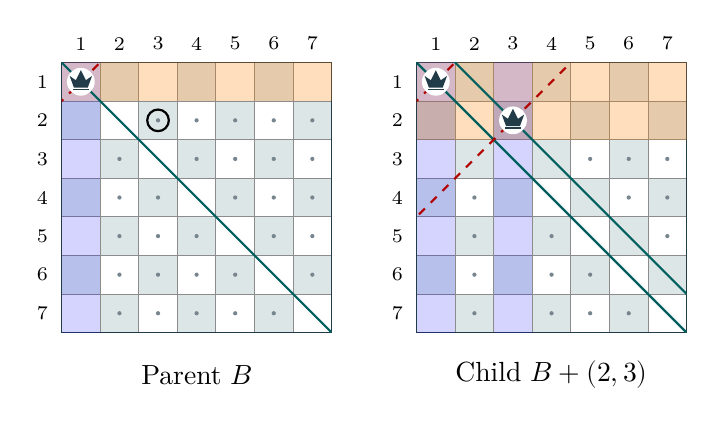
\begin{tikzpicture}[x=.49cm,y=.49cm]
 \foreach \etapa/\dx in {1/0,2/9.2}{
  \begin{scope}[shift={(\dx,0)}]
   \bcuadricula{7}
   \fill[orange,opacity=.26] (0,6) rectangle (7,7);
   \fill[blue,opacity=.17] (0,0) rectangle (1,7);
   \ifnum\etapa=2
    \fill[orange,opacity=.26] (0,5) rectangle (7,6);
    \fill[blue,opacity=.17] (2,0) rectangle (3,7);
   \fi
   \begin{scope}
    \clip (0,0) rectangle (7,7);
    \draw[teal!75!black,line width=.8pt] (.5,6.5) ++(-7,7) -- ++(14,-14);
    \draw[red!70!black,dashed,line width=.8pt] (.5,6.5) ++(-7,-7) -- ++(14,14);
    \ifnum\etapa=2
     \draw[teal!75!black,line width=.8pt] (2.5,5.5) ++(-7,7) -- ++(14,-14);
     \draw[red!70!black,dashed,line width=.8pt] (2.5,5.5) ++(-7,-7) -- ++(14,14);
    \fi
   \end{scope}
   \foreach \rr in {1,...,7}{
    \foreach \cc in {1,...,7}{
     \pgfmathtruncatemacro{\libre}{(\rr!=1)&&(\cc!=1)&&(abs(\rr-1)!=abs(\cc-1))}
     \ifnum\etapa=2
      \pgfmathtruncatemacro{\libre}{\libre&&(\rr!=2)&&(\cc!=3)&&(abs(\rr-2)!=abs(\cc-3))}
     \fi
     \ifnum\libre=1 \bmarca{7}{\rr}{\cc}\fi
    }
   }
   \breina{7}{1}{1}
   \ifnum\etapa=1
    \draw[black,line width=.8pt] (2.5,5.5) circle[radius=.28];
    \node at (3.5,-1.1) {Parent $B$};
   \else
    \breina{7}{2}{3}
    \node at (3.5,-1.1) {Child $B+(2,3)$};
   \fi
  \end{scope}
 }
\end{tikzpicture}
\caption{One transition from a parent to a child on a board of order seven. The parent has a queen
in row 1; the child is obtained by revealing row 2.
Rows are numbered from one, top to bottom, and columns from one, left to right. Crowns represent
queens already placed. The horizontal and vertical bands mark their occupied rows and columns.
Solid and dashed lines show the two families of diagonals under attack. Each dot marks an available
square. In the next row, row $2$, columns $3,4,5,6,7$ have $1,1,1,1,0$ completions, respectively,
so $Q(B)=4$. The circle marks the choice $(2,3)$ that gives the child on the right.}\label{fig:historia}
\end{figure}


\paragraph{Profile and normalization.}
Theorem~1.1 of~\cite{perfil} gives the unique optimal profile of mass one, $\nu_1$, on the unit square. We
denote its entropy by $s_1$ and write $\Phi=s_1+1$. As in~\cite{perfil,ultimas,pred}, $m_D$ and $m_A$ are
the projections of $\nu_1$ onto the two diagonal families, and $u_D=1-m_D$, $u_A=1-m_A$ are their
vacancies. For a diagonal line $f$, $m_f$ and $u_f$ denote the values at $f$ of the functions for its
family. Theorems~1.2 and~1.3 and Proposition~5.2 of~\cite{perfil} identify the positive factors and the
limit at mass one. Theorem~7.7 of the same work gives control up to the endpoint. We use the form given
in~\cite[Section~2]{pred},
\[
 \nu_1(r,c)=b_0 r_R(r)r_C(c)u_D(r-c)u_A(r+c),\qquad
 c_\nu\le\nu_1\le C_\nu,\quad \kappa_\nu\le u_D,u_A\le1.
\]
The row and column marginals of $\nu_1$ are equal to one, the factors are Lipschitz, and $L_\nu$ denotes a
Lipschitz constant for $\nu_1$, as in~\cite{pred}. The continuous coordinates of the square $(i,j)$ are
those of the center of its cell of side length $1/n$.

\paragraph{Bethe point and predictor.}
We use RC for rows and columns. As in~\cite{pred}, the \emph{Bethe point} of a residual board $B$ is the
vector $p=(p_e)$, with one weight per square in $E(B)$, at which its predictor is evaluated. It is the
stationary point of the Bethe entropy
\begin{equation}\label{bethe}
 H_B(p)=-\sum_e p_e\log p_e
       +3\sum_e(1-p_e)\log(1-p_e)-\sum_fh_f\log h_f
\end{equation}
on the domain $0<p_e<1/4$, $h_f>0$, with row and column masses equal to one. Here the \emph{mass} of a
diagonal $f$ is $\ell_f=\sum_{e\in f}p_e$, and its \emph{vacancy} is $h_f=1-\ell_f$. Physical availability
is an indicator distinct from this vacancy. On this domain $-H_B$ is strictly convex, so there is at most
one stationary point. We use the Bethe point only on the regular boards of Definition~\ref{def:regular}
and on their children, where it exists.

Suppose the row--column graph of the support is connected. Let $S_B$ be the line operator given in
Section~\ref{costes:normalizador}, and let $\pdet$ denote the product of the nonzero eigenvalues. The
predictor satisfies
\[
 L(B)=H_B(p)-\tfrac12\sum_e[\log(1-4p_e)-4\log(1-p_e)]
             -\tfrac12\log\pdet S_B+\tfrac12\log(4\pi k).
\]
The zero mode of $S_B$ is proportional to $(\mathbf1_R,-\mathbf1_C,0)$; it is the gauge of~\cite{pred}.
Deleting the row and column of $S_B$ for the same RC line gives a cofactor equal to $\pdet S_B/(2k)$,
since the corresponding component of the unit zero-mode vector has square $1/(2k)$. Thus using this
cofactor with $\tfrac12\log(2\pi)$, as in~\cite[Sections~6.1 and~7.1]{pred}, gives the same $L(B)$.

As in~\cite{pred}, the \emph{row--column Laplacian} of $p$ is the Laplacian of the graph whose vertices
are the empty rows and columns, with an edge of weight $p_e$ joining the row and column of each available
square $e$. Its \emph{gap} is its second-smallest eigenvalue. We say that $p$ satisfies a \emph{diffusion
bound} if $k\max_ep_e\le C$, that is, if no weight exceeds $C/k$; a \emph{vacancy bound} if $h_f\ge\eta$
on every diagonal; and a \emph{gap bound} if the gap is at least $\gamma$. For fixed constants
$C,\eta,\gamma>0$, these are the bounds required by Theorems~7.1 and~8.1 of~\cite{pred}. The former
assumes $k\ge\delta n$, and the latter dispenses with that condition if each diagonal has mass at most a
small $\varepsilon$.

Some notation differs from that of~\cite{pred}. There the child is written $B+c$, the row is implicit in
the ratio $\rho(B)$, which we write as $\rho(B,i)$, and the mass and vacancy of a diagonal are $m_d$ and
$h_d$. We indicate other differences as they arise. In some sections, letters such as $B$, $E$, $J$, $S$,
$T$, or $W$ denote objects defined locally. For example, in Section~\ref{permanente} the letter $B$
denotes the matrix $P-J_K$ rather than a board. Outside the abstract and introduction, $J$ does not denote
the operator of~\cite{pred}.

Some Greek letters have two uses that must not be confused. The letter $\nu$ without a subscript is
the adaptive law, whereas $\nu_1$ is always the profile and $c_\nu,C_\nu,\kappa_\nu,L_\nu$ are its
constants. The letter $\tau$ alone is the stopping time of Section~\ref{historias}, whereas $\tau_d$
and $\tau_e$, always with a subscript, are the weights of Section~\ref{costes:normalizador}. The
letter $\alpha$ alone is the constant of the introduction; the geometric threshold of
Section~\ref{meso} is written $\alpha_{\rm geo}$. In Lemma~\ref{terminal-escalado}, $\alpha$ and
$\beta$ are scaling vectors, unrelated to that constant and to the function $\beta$ of
Section~\ref{meso:constantes}.
Likewise, $F$ without arguments is the permanence event, whereas $F_{\lambda,I}$, $F_i(k)$,
$F(\sigma)$ and $F(x)$ are local objects of Sections~\ref{macro:observaciones}, \ref{meso},
\ref{costes:permanente} and~\ref{meso:regularidad}.

\paragraph{Laws for revealing and inserting queens.}
We draw a uniformly random ordering $\sigma$ of the rows. Under the \emph{uniform law} $\mu$, we choose a
uniform solution independently of $\sigma$ and reveal its queens in that order. Under the \emph{adaptive
law} $\nu$, given the next row $i$, we choose $e$ with probability
\[
 \nu_B(e\mid i)=\frac{\exp L(B+e)}{\sum_{e'\in R_i\cap E(B)}\exp L(B+e')},\qquad
 \rho(B,i)=\sum_{e'\in R_i\cap E(B)}\exp\{L(B+e')-L(B)\}.
\]
The \emph{auxiliary law} $P^{\rm B}$ uses the same uniformly chosen row and selects $e$ with
probability $p_e$. In $P^{\rm B}$ and in its expectation $\E_{\rm B}$, the upright B stands for
Bethe and does not denote a board. A \emph{history} is the resulting sequence of boards
$B_0,B_1,\dots$ together with the row order. A board with $k$ empty rows has \emph{size} $k$.
We index $B_t$ and the revealed history $\mathcal F_t$ by the number $t$ of insertions.
When indexing by size we use $B^{(k)}=B_{n-k}$ and $\mathcal F^{(k)}=\mathcal F_{n-k}$.
The latter contains the rows revealed so far and their chosen squares, before the next row is
revealed. On a stopped history these symbols refer only to levels that have been reached.

\section{Two comparisons on stopped histories}\label{historias}
Let $\tau$ be a stopping time that uses only the row order and the information revealed through the current
step. Suppose every parent before the stopping time and each of its children have a finite predictor. Write
$B_t$ for the board in the history after $t$ insertions and $i_t$ for the next row to be revealed. Write
$\omega$ for the prefix of squares, including the last insertion, $B_\tau$ for its residual board, and
$\mu^\tau,\nu^\tau$ for the joint laws of the order and the prefix. Define
\[
 A_\tau=\sum_{t<\tau}\log\rho(B_t,i_t),\qquad g(B)=\log Q(B)-L(B)\quad(Q(B)>0).
\]

\begin{lema}[Comparison at the first stopping time]\label{hist:igualdad}
If $Q(B_0)>0$, then $\mu^\tau\ll\nu^\tau$ and
\begin{equation}\label{super}
 g(B_0)=\E_\mu[A_\tau+g(B_\tau)]-D(\mu^\tau\Vert\nu^\tau).
\end{equation}
Here $D$ is the relative entropy of the two discrete laws.
\end{lema}
\begin{proof}
For a fixed order $\sigma$, each of the $Q(B_\tau)$ completions extends the prefix in exactly one way. Under
$\nu$ we multiply the probabilities of choosing the successive squares. The differences of the predictors
telescope. Thus the two masses at the same atom are
\[
 \mu^\tau(\sigma,\omega)=\frac{Q(B_\tau)}{n!\,Q(B_0)},\qquad
 \nu^\tau(\sigma,\omega)=\frac{\exp\{L(B_\tau)-L(B_0)-A_\tau\}}{n!}.
\]
The second mass is positive on the support of the first. Taking the logarithm of their ratio in the order
$\mu^\tau/\nu^\tau$ gives $A_\tau+g(B_\tau)-g(B_0)$. By definition, its mean under $\mu^\tau$ is the
relative entropy in \eqref{super}.
\end{proof}

\begin{proposicion}[Lower bound from permanence]\label{hist:inferior}
Let $\tau$ be the stopping time of Definition~\ref{def:regular}, namely the first exit or, if there is none,
the time at which the board reaches size $K$. Let $F$ be the permanence event and $B_K$ the board of size
$K$, so that $B_K=B_\tau$ on $F$. The subscript of $B_K$ counts empty rows rather than steps. Let
$G=F\cap\{Q(B_K)>0\}$. If $s=\nu(G)>0$, then
\begin{equation}\label{infer}
 g(B_0)\ge \E_{\nu(\cdot\mid G)}[A_\tau+g(B_K)]+\log s.
\end{equation}
\end{proposicion}
\begin{proof}
For each order, distinct stopped prefixes have disjoint sets of completions. For each history in $G$,
multiplying its mass under $\nu^\tau$ by $\exp\{A_\tau+g(B_K)\}$ gives $Q(B_K)e^{-L(B_0)}/n!$. Summing first
over prefixes and then over orders gives
\[
 \int_G\exp\{A_\tau+g(B_K)\}\,d\nu^\tau\le Q(B_0)e^{-L(B_0)} .
\]
The integral is $s$ times the conditional expectation of the exponential. Concavity of the logarithm gives
\eqref{infer}, even when conditioning changes the distribution of the order.
\end{proof}

\begin{corolario}[Cumulative consistency]\label{hist:consistencia}
Suppose each parent before the stopping time satisfies the hypotheses of Theorem~7.1 and Corollary~7.2
of~\cite{pred} for $k>M=\lceil\delta n\rceil$, and those of Theorem~8.1 of the same work for $K<k\le M$.
Then $|A_\tau|\le C/K+O_\delta(n^{-1})$ uniformly over histories.
\end{corolario}
\begin{proof}
These results give $|\log\rho(B,i)|\le C_*/k^2$ in each row, with all the children in that row included in
$\rho$. For parents with $k>M$, the constant depends on $\delta$ and the diffusion, vacancy, and gap bounds.
For parents with $K<k\le M$, it depends on the constants of the weak class of~\cite[Section~8.1]{pred}. A
regular parent in the sense of Definition~\ref{def:regular} belongs to the inner class, by definition if
$k<M$ and by Proposition~\ref{meso:reconstruccion} if $k=M$. The sum of $k^{-2}$ over $k>m$ is at most
$\int_m^\infty t^{-2}\,dt=1/m$. A history that stops earlier uses a subset of these summands.
\end{proof}

\section{Permanence while at least \texorpdfstring{$\delta n$}{δn} rows remain}\label{macro}
The goal of this section is Corollary~\ref{macro:cambio}: under the adaptive law $\nu$, except with
probability exponentially small in $n$, every board of the history down to size
$M=\lceil\delta n\rceil$ has a Bethe point that is the unique maximizer and satisfies uniform
diffusion, vacancy, and gap bounds. We prove this first under the auxiliary law $P^{\rm B}$. We
compare the history with a deterministic trajectory (Proposition~\ref{macro:trayectoria}) by means
of observations of rows, columns, fibers, and rectangles (Section~\ref{macro:observaciones}). These
observations allow us to reconstruct the Bethe point (Proposition~\ref{macro:maximo}) and
concentrate around their targets (Proposition~\ref{macro:parada}). Passing from $P^{\rm B}$ to
$\nu$ costs a bounded factor. Comparing a discrete process with the solution of a differential
system, by means of martingales, follows the scheme of Wormald's differential equation
method~\cite{wormald}.

\subsection{Exposure process and comparison trajectory}

Fix $0<\delta<1$. After $s$ choices, write $k=n-s$, $x=k/n$, and $t=s/n$. Under $P^{\rm B}$, we
reveal the uniform random permutation $\sigma$ of the rows one row at a time. Conditional on the
history $\mathcal F_s$ of the choices and the rows already revealed, the next row is uniform among
the $k$ empty rows. If $p$ is the Bethe point of the current board, the conditional probability of
selecting a square $e$ is $p_e/k$. We set $p_e=0$ on squares outside the support. The discrete
indices run from $1$ to $n$. The physical centers $r_i=(i-\tfrac12)/n$ and $c_j=(j-\tfrac12)/n$
place the diagonal $D(e)=i-j$ at $r_i-c_j$ and the antidiagonal $A(e)=i+j-1$ at $r_i+c_j$.
Let $X_f$ denote the availability indicator of a line and $Y_e=\prod_{f\ni e}X_f$ that of a square.
As in Section~\ref{leyes}, $\ell_f$ and $h_f$ are the mass and vacancy of a diagonal or antidiagonal
$f$ at the point $p$.

\begin{lema}[Loss of a square]\label{macro:casilla}
The conditional probability of occupying a given available row or column is $1/k$. The probability of
occupying a given available diagonal $f$ is $\ell_f/k$. For $e=(i,j)$ we have
\[
 \E_{\rm B}[Y_e(s+1)-Y_e(s)\mid\mathcal F_s]
 =-\frac{Y_e(s)}{k}\bigl(2+\ell_{D(e)}+\ell_{A(e)}-3p_e\bigr).
\]
\end{lema}
\begin{proof}
Summing $p_e/k$ over the corresponding line gives the first two formulas. If $Y_e=1$, the four
lines through $e$ intersect only at that square. The sum of their masses counts $e$ four times, and
it must be counted once. If $Y_e=0$, no choice can make the square available again.
\end{proof}

On the unit square we use the profile
\[
 \nu_1(r,c)=b_0r_R(r)r_C(c)u_D(r-c)u_A(r+c).
\]
Its row and column marginals are both one. For $d\in[-1,1]$ and $a'\in[0,2]$, its projections onto
the two diagonal families, that is, the masses of its fibers, are
\[
 m_D(d)=\int_{\{0\le r,r-d\le1\}}\nu_1(r,r-d)\,dr,\qquad
 m_A(a')=\int_{\{0\le r,a'-r\le1\}}\nu_1(r,a'-r)\,dr .
\]
Here and below, the notation under the integral sign requires both coordinates to belong to $[0,1]$.
The vacancies are $u_f=1-m_f$. We use the bounds $c_\nu\le\nu_1\le C_\nu$ and $u_f\ge\kappa_\nu>0$
and the Lipschitz regularity of the full-board profile \cite[Theorems~1.1--1.3, Proposition~5.2 and
Theorem~7.7]{perfil}. The fiber masses are Lipschitz in their parameter. Indeed, shifting the
parameter by $\epsilon$ moves each endpoint of integration by at most $|\epsilon|$ and changes the
integrand on the overlap by at most $L_\nu|\epsilon|$.

The following proposition gives the deterministic targets against which we compare the process when
a fraction $x$ of the rows remain. For a diagonal $f$, $U_f(x)$ is the target for its availability
indicator and $\ell_f^*(x)$ is the target for its mass. At a point $(r,c)$, $J_x$ is the target for
the availability indicator of the square and $v_x/n$ is the target for the Bethe weight of an
available square.

\begin{proposicion}[Comparison trajectory]\label{macro:trayectoria}
For a diagonal line $f$, a point $(r,c)$, and $0\le x\le1$, write
\begin{gather*}
 U_f(x)=u_f+xm_f,\qquad \ell_f^*(x)=\frac{xm_f}{U_f(x)},\\
 J_x=x^2U_D(x)U_A(x),\qquad
 W_x=\frac{\nu_1}{U_D(x)U_A(x)}.
\end{gather*}
Subscripts $D,A$ without arguments indicate evaluation at $r-c,r+c$, respectively. Since $u_f\ge
\kappa_\nu$, $W_x$ is continuous down to $W_0=\nu_1/(u_Du_A)=b_0r_Rr_C$, the weight used in
Section~\ref{meso:regularidad}. We have $J_1=1$. For $0<x\le1$, set $v_x=W_x/x$. Then
$J_xv_x=x\nu_1$, both marginals of $J_xv_x$ are equal to $x$, and
\begin{equation}\label{macro:derivadas}
 \partial_t U_f=-\frac{\ell_f^*}{x}U_f,\qquad
 \partial_t\log J_x=-\frac{2+\ell_D^*+\ell_A^*}{x},\qquad
 1-\ell_f^*=\frac{u_f}{U_f}\ge\kappa_\nu .
\end{equation}
In particular,
\[
 v_x=\frac{b_0}{x}\,r_Rr_C\frac{u_D}{U_D}\frac{u_A}{U_A},
 \qquad xv_x\le C_\nu/\kappa_\nu^2 .
\]
\end{proposicion}
\begin{proof}
We have $U_f(1)=1$, $\kappa_\nu\le U_f(x)\le1$, and $dx/dt=-1$. Hence $\partial_t U_f=-m_f$.
Differentiating the product defining $J_x$ gives the second identity in \eqref{macro:derivadas}.
Substituting the factorization of $\nu_1$ gives the formula for $v_x$. The product identity and the
claims about the marginals follow by integration.
\end{proof}

The comparison that follows requires products of availability indicators for several lines.
Observing the two diagonal families separately gives only the means of the individual factors.
We now define sums of products and prove their concentration without assuming independence of the
lines.

\subsection{Observations on intervals, fibers, and rectangles}\label{macro:observaciones}

Take a partition $\mathcal I$ of $[0,1]$ into intervals of length at most $a_{\rm mac}$, assigning
each endpoint to a single interval. We may take all intervals to have equal length. An index belongs
to the interval containing its physical center. For rows and columns we record
\[
 N^R_I=\frac1n\sum_{r_i\in I}X_{R_i},\qquad
 N^C_I=\frac1n\sum_{c_j\in I}X_{C_j},\qquad
 N^{R,*}_I=N^{C,*}_I=x|I|.
\]
The fiber parameter is $c$ on a row and $r$ on a column, diagonal, or antidiagonal. Fix a line
$\lambda$, called the \emph{tracked line}, whose fiber we observe. For an interval $I$, write
$\lambda_I$ for the part of the physical fiber whose parameter belongs to $I$, and $dz$ for the
parameter measure. There is no Euclidean length factor on oblique fibers, since there are $n$
indices per unit of $r$.

\begin{definicion}[Fiber observations]\label{macro:fibras}
While $\lambda$ is available, its observation is
\[
 F_{\lambda,I}=\frac1n\sum_{e\in\lambda_I}
                  \prod_{f\ni e,\ f\ne\lambda}X_f .
\]
For each of the four families, the target $F^*_{\lambda,I}$ is the integral over $\lambda_I$ of the
density in the second column of the table. The last column gives the sum of the rates for the three
lines in the product, before division by $x$.
\[
\begin{array}{c|c|c}
 \lambda & \text{target density} & H^*_{\lambda}(e)\\ \hline
 R_i & xU_DU_A  & 1+\ell_D^*+\ell_A^*\\
 C_j & xU_DU_A  & 1+\ell_D^*+\ell_A^*\\
 D_d & x^2U_A   & 2+\ell_A^*\\
 A_{a'} & x^2U_D & 2+\ell_D^*
\end{array}
\]
If the choice at a step occupies $\lambda$, we retain the values of $F_{\lambda,I}$ and
$F^*_{\lambda,I}$ immediately before that step and hold them constant thereafter. We call this the
\emph{freezing rule}. The balances in Lemma~\ref{macro:balances} use only lines that are still
available.
\end{definicion}

Order the positions of a rectangle as
$e_1=(i,j)$, $e_2=(i',j)$, $e_3=(i',j')$, $e_4=(i,j')$.
Call a quadruple $(i,i',j,j')$ ordinary if $i\ne i'$, $j\ne j'$, and the four labels within each
diagonal family are pairwise distinct. There are $O(n^3)$ remaining quadruples. Each forbidden
equality is a nontrivial linear equation in four indices. Fixing three suitably chosen indices
determines the fourth, and there are only a fixed number of equalities. This estimate also covers
the edges of the board.

\begin{definicion}[Rectangle observations]\label{macro:rectangulos}
For $T\subseteq\{1,2,3,4\}$ and a box $\Theta\in\mathcal I^4$, we track the sum and its target
\begin{align*}
 P_{\Theta,T}&=\frac1{n^4}
 \sum_{(i,i',j,j')\in\Theta}^{\rm ord}
 X_{R_i}X_{R_{i'}}X_{C_j}X_{C_{j'}}
 \prod_{m\in T}X_{D(e_m)}X_{A(e_m)},\\
 P^*_{\Theta,T}&=\int_\Theta x^4\prod_{m\in T}U_{D(e_m)}U_{A(e_m)}
                  \,dr\,dr'\,dc\,dc'.
\end{align*}
The four continuous coordinates determine the positions in the integral. The pattern for
$T=\varnothing$ counts only the two rows and two columns. Individual rectangles cease to contribute
when they lose a line.
\end{definicion}

We measure the discrepancies by
\begin{align*}
 \Delta_0&=\sum_{I\in\mathcal I}
   (\bigl|N^R_I-x|I|\bigr|+\bigl|N^C_I-x|I|\bigr|),\\
 \Delta_F&=\max_{\lambda}\sum_{I\in\mathcal I}|F_{\lambda,I}-F^*_{\lambda,I}|,\\
 \Delta_R&=\sum_{\Theta\in\mathcal I^4}\ \sum_{T\subseteq\{1,2,3,4\}}
                      |P_{\Theta,T}-P^*_{\Theta,T}|,\qquad
 \Delta=\Delta_0+\Delta_F+\Delta_R .
\end{align*}
In the first line, $x|I|$ is the target mass of each interval. We write $C_{\mathcal I}$ for constants
that may depend on the fixed partition $\mathcal I$, and set
\[
 \zeta=\Delta_0+\Delta_F+a_{\rm mac}+C_{\mathcal I}/n .
\]
On the $k$ available rows and $k$ available columns, consider
\[
 q_{ij}=\frac{Y_{ij}\nu_1(r_i,c_j)}{kU_{D(i,j)}U_{A(i,j)}},\qquad
 V_{ij}=\frac{\nu_1(r_i,c_j)}k .
\]
The factors $U$ are evaluated at $x$, so $q_{ij}=Y_{ij}W_x(r_i,c_j)/k=Y_{ij}v_x(r_i,c_j)/n$.
The matrix $q$ is our explicit candidate for the Bethe point. Proposition~\ref{macro:maximo} proves
that $p_e/q_e$ is close to one on available squares. Replacing $Y_{ij}$ in $q$ by $U_DU_A$, its
target when the row and column are available, gives the matrix $V$.

Figure~\ref{fig:rectangulo} shows two selected positions and their corresponding sign.
\begin{figure}[htbp]
\centering
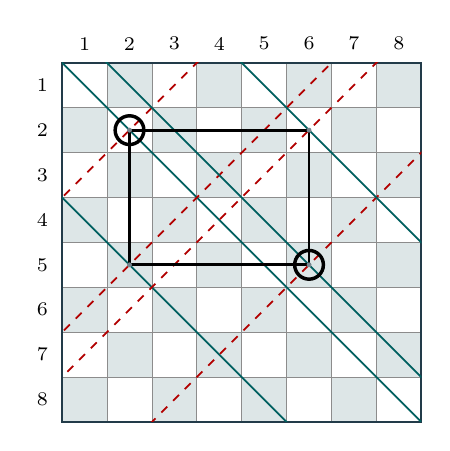
\begin{tikzpicture}[x=.57cm,y=.57cm]
 \bcuadricula{8}
 \begin{scope}
  \clip (0,0) rectangle (8,8);
  \foreach \rr/\cc in {2/2,5/2,5/6,2/6}{
   \draw[teal!75!black,line width=.65pt] ({\cc-.5},{8.5-\rr}) ++(-8,8) -- ++(16,-16);
   \draw[red!70!black,dashed,line width=.65pt] ({\cc-.5},{8.5-\rr}) ++(-8,-8) -- ++(16,16);
  }
 \end{scope}
 \draw[black,line width=1pt] (1.5,6.5) rectangle (5.5,3.5);
 \foreach \rr/\cc in {2/2,5/2,5/6,2/6}{\bmarca{8}{\rr}{\cc}}
 \draw[black,line width=1.25pt] (1.5,6.5) circle[radius=.32];
 \draw[black,line width=1.25pt] (5.5,3.5) circle[radius=.32];
\end{tikzpicture}
\caption{A rectangle on an empty board of order eight. Rows are numbered from one, top to bottom,
and columns from one, left to right. The vertices, in order, are $e_1=(2,2)$, $e_2=(5,2)$,
$e_3=(5,6)$ and $e_4=(2,6)$. Four diagonals $i-j$ (solid) and four antidiagonals $i+j-1$ (dashed)
pass through them. The circles select the opposite vertices $e_1,e_3$. The term in the expansion with
$T=\{1,3\}$ has sign $(-1)^{4-2}=+1$.}\label{fig:rectangulo}
\end{figure}


\begin{lema}[Interval and fiber balances]\label{macro:balances}
For $k\ge\delta n$, the row and column sums of $V$ differ from one by
$O_\delta(\Delta_0+a_{\rm mac}+C_{\mathcal I}/n)$. For $q$, the row and column sums differ from one
and the masses on available diagonal lines differ from $\ell_f^*$ by
$O_\delta(\Delta_F+a_{\rm mac}+C_{\mathcal I}/n)$, uniformly over the lines.
\end{lema}
\begin{proof}
On each interval we replace the weight by its value at a point of the physical region of integration.
The weights $\nu_1$ and $W_x=\nu_1/(U_DU_A)$ are uniformly bounded and Lipschitz. The error of this
replacement, summed over the intervals of a line, is $O_\delta(a_{\rm mac})$, since the variation in
the weight multiplies the sum of the masses on that line. The error in the weighted masses is at
most the supremum norm of the weight times the sum of the absolute discrepancies. Converting $1/n$
to $1/k$ contributes a factor $1/x$. For $V$, the target for a row is
$x^{-1}\int\nu_1(r,c)x\,dc=1$, and the same holds for columns. On an available row, the three
indicators in the fiber observable give $Y_{ij}$, and its target weighted mass is
\[
 \frac1x\int_0^1 \frac{\nu_1}{U_DU_A}\,xU_DU_A\,dc=1.
\]
The same calculation with $dr$ gives the column sum. For diagonal $d$, the target is
\[
 \frac1x\int_{D_d}\frac{\nu_1}{U_DU_A}\,x^2U_A\,dr
 =\frac{xm_D(d)}{U_D(d)} .
\]
Interchanging $D$ and $A$ for an antidiagonal gives $xm_A/U_A$. Endpoint or Riemann sum
approximations on the fixed partition incur an error of at most $C_{\mathcal I}/n$.
\end{proof}

\begin{lema}[Cancellation of the sixteen terms and the gap]\label{macro:brecha}
For $E=q-V$ we have
\[
 \|E\|_{\rm op}\le C_\delta(\Delta_R+a_{\rm mac}+C_{\mathcal I}/n)^{1/4}.
\]
If $\Delta$, $a_{\rm mac}$, and $C_{\mathcal I}/n$ are sufficiently small in terms of $\delta$ and
the profile, then the row--column Laplacian with weights $q$ has gap at least $c_\nu/2$ on the
orthogonal complement of the constant vector.
\end{lema}
\begin{proof}
By the singular value bound and the trace expansion,
\[
 \|E\|_{\rm op}^4\le {\rm tr}((EE^T)^2)
 =\sum_{i,i',j,j'}E_{ij}E_{i'j}E_{i'j'}E_{ij'} .
\]
From the summand we can factor out the indicator that all four row and column lines are available,
together with $k^{-4}\prod_m\nu_1(e_m)$. The remaining factor is $\prod_{m=1}^4(B_m-1)$, where

\[ B_m=\frac{X_{D(e_m)}X_{A(e_m)}}{U_{D(e_m)}U_{A(e_m)}}. \]
Writing $B_T=\prod_{m\in T}B_m$ and listing the elements of each index set as subscripts, we obtain
the full expansion
\[
 \begin{aligned}
 1
 &-(B_1+B_2+B_3+B_4)\\
 &+(B_{12}+B_{13}+B_{14}+B_{23}+B_{24}+B_{34})\\
 &-(B_{123}+B_{124}+B_{134}+B_{234})+B_{1234}.
 \end{aligned}
\]
The exceptional quadruples contribute $O_\delta(1/n)$ in total, since each product is
$O_\delta(k^{-4})$. For each ordinary term, the weight multiplying the pattern of
Definition~\ref{macro:rectangulos} in the sum normalized by $n^4$ is
\[
 W_T=x^{-4}\frac{\prod_m\nu_1(e_m)}
                 {\prod_{m\in T}U_{D(e_m)}U_{A(e_m)}} .
\]
Its supremum norm and Lipschitz constant are bounded in terms of $\delta$ and the profile. Replacing
it by a constant on each box incurs a total error of $O_\delta(a_{\rm mac})$, since for each $T$ the
masses of all boxes sum to at most one. Replacing the discrete masses by their targets then incurs
an error of $O_\delta(\Delta_R)$. Restoring the variable weight in the integral gives the same
weighted target density $\prod_m\nu_1(e_m)$ for each of the sixteen terms. Its total coefficient is
therefore $1-4+6-4+1=0$. This proves the norm estimate.

Let $V'=V-c_\nu\mathbf1\mathbf1^T/k$. Its entries are nonnegative, and its row and column sums are
at most $1-c_\nu+O_\delta(\zeta)$ by Lemma~\ref{macro:balances}. The Schur bound gives the same
upper bound for $\|V'\|_{\rm op}$. If $(u,v)\perp\mathbf1_{2k}$, then $(\sum_i u_i)(\sum_j
v_j)=-(\sum_i u_i)^2\le0$. The constant matrix thus contributes a nonnegative term to the quadratic
form of the Laplacian. The degrees on the diagonal are $1+O_\delta(\zeta)$, and
$2\|u\|_2\|v\|_2\le\|u\|_2^2+\|v\|_2^2$. The resulting lower bound for the quadratic form is
\[
 \bigl(c_\nu-O_\delta(\zeta)-\|E\|_{\rm op}\bigr)
                   (\|u\|_2^2+\|v\|_2^2).
\]
Reducing the three thresholds gives the claimed gap. The exponent $1/4$ is used only to guarantee
this gap.
\end{proof}

\subsection{Reconstruction of the Bethe point}\label{macro:reconstruccion}
Throughout this subsection we assume $k\ge\delta n$, as in Lemma~\ref{macro:balances}.

\begin{proposicion}[Row and column rebalancing]\label{macro:reequilibrado}
Under the thresholds of Lemma~\ref{macro:brecha}, there exists a matrix $\bar p$ with the same
support as $q$, with row and column sums exactly equal to one, and with
\[
 \max_{q_e>0}\left|\frac{\bar p_e}{q_e}-1\right|\le C_\delta\zeta .
\]
Its diagonal vacancies are at least $\kappa_\nu/2$, its entries are $O_\delta(1/k)$, and its
row--column Laplacian retains a uniform positive gap.
\end{proposicion}
\begin{proof}
Restrict the variables to the available squares, where $q_e>0$. Let $B$ be the incidence matrix
with rows indexed by row and column lines and columns indexed by squares. As
in~\cite[Section~6.1]{pred}, $B$ here denotes this matrix rather than a board. Let $J$ be the
diagonal matrix that changes the sign of the column coordinates, and set $B_o=JB$. For
$b=\mathbf1-Bq$ we have $\|b\|_\infty=O_\delta(\zeta)$ and $\mathbf1^TJb=0$, since the sum of the
row masses equals the sum of the column masses. With $L_q$ the row--column Laplacian with weights
$q$, define
\[
 L_q=B_o\operatorname{diag}(q)B_o^T,\qquad
 \phi=L_q^+Jb,\qquad z=\operatorname{diag}(q)B_o^T\phi .
\]
The gap and the compatibility condition give $Bz=b$ and $\|\phi\|_2\le C_\delta\sqrt{k}\,\zeta$.
At a graph vertex $\gamma$, that is, a row or column, the equation $L_q\phi=Jb$ and the degree
$d_\gamma=1+O_\delta(\zeta)$ give
\[
 d_\gamma|\phi_\gamma|\le |b_\gamma|+
 \left(\sum_{e\in\gamma}q_e^2\right)^{1/2}\|\phi\|_2,
 \qquad \sum_{e\in\gamma}q_e^2\le \frac{C_\delta}{k}d_\gamma .
\]
Thus $\|\phi\|_\infty=O_\delta(\zeta)$ and $|z_e|/q_e\le2\|\phi\|_\infty$. Take $\bar p=q+z$. The
multiplicative comparison of weights preserves a fixed fraction of the gap of $L_q$. It also changes
each diagonal mass by $O_\delta(\zeta)$ by Lemma~\ref{macro:balances}. By \eqref{macro:derivadas},
the target vacancies are at least $\kappa_\nu$, which gives the bounds in the proposition upon
reducing the thresholds.
\end{proof}

\begin{lema}[Inverse on the tangent space at the feasible point]\label{macro:inversa}
For $\bar p$ as in Proposition~\ref{macro:reequilibrado}, let $K_{\bar p}$ denote the negative
Hessian of the Bethe entropy at $\bar p$, and let $Z$ be a matrix whose orthonormal columns span
$\ker B$. For large $n$,
\[
 R=Z(Z^TK_{\bar p}Z)^{-1}Z^T,\qquad
 \|\operatorname{diag}(\bar p)^{-1}R\|_{\infty\to\infty}\le C_\delta .
\]
\end{lema}
\begin{proof}
We give the matrix argument of \cite[Sections~6.3, 6.4 and~7.2]{pred} at this feasible point. Let $D$ be
the square--diagonal incidence matrix for both diagonal families, as in~\cite[Section~6.1]{pred}.
The letter $D$ alone denotes this matrix, and $D(e)$ still denotes the diagonal of square $e$. Let
$H=\operatorname{diag}(h_f(\bar p))$ and
\[
 w_e=\left(\frac1{\bar p_e}-\frac3{1-\bar p_e}\right)^{-1},
 \qquad W=\operatorname{diag}(w_e),\qquad
 K_{\bar p}=W^{-1}+DH^{-1}D^T .
\]
We have $w_e/\bar p_e=1+O_\delta(1/k)>0$. If $\Upsilon$ is formed by stacking $B_o$ and $D^T$, the
system for $v=R\psi$ is equivalent to
\begin{equation}\label{macro:sistema-inverso}
 (\Upsilon W\Upsilon^T+\operatorname{diag}(0,H))\,y=\Upsilon W\psi,\qquad
 v=W(\psi-\Upsilon^Ty).
\end{equation}
Indeed, the first block gives $B_ov=0$ and the second gives $D^Tv=Hy_D$, where $y_D$ collects both
diagonal families. Thus $K_{\bar p}v=\psi-B_o^Ty_{RC}$.

We solve \eqref{macro:sistema-inverso} with $y_{RC}\perp\mathbf1_{2k}$, a condition compatible with
the first block. The quadratic form of the system matrix is
\[
 \|W^{1/2}(B_o^Ty_{RC}+Dy_D)\|_2^2+y_D^THy_D .
\]
Its second term dominates $\kappa_\nu\|y_D\|_2^2/2$. Moreover,
$\|W^{1/2}Dy_D\|_2^2\le 2\max_f\sum_{e\in f}w_e\,\|y_D\|_2^2$,
since each square is incident to two diagonals. The gap of $B_oWB_o^T$ and the triangle inequality
then show that the form also dominates a positive constant times $\|y_{RC}\|_2^2$. The entries of
$\Upsilon W\psi$ are bounded by $C_\delta\|\psi\|_\infty$, and there are at most $2k+4n$ lines.
Coercivity gives $\|y\|_2\le C_\delta\sqrt{k}\|\psi\|_\infty$.

Each main diagonal entry of the system matrix is bounded away from zero by the row and column sums
or by $H$. Two distinct lines intersect in at most one square. Thus each off-diagonal entry has
absolute value at most $\max_e w_e=O_\delta(1/k)$, and in each row the sum of their absolute values
is at most three times the weighted degree of the line, which is $O_\delta(1)$. The Euclidean norm
of the off-diagonal part of each row is therefore $O_\delta(k^{-1/2})$. Applying the equation
coordinate by coordinate gives $\|y\|_\infty\le C_\delta\|\psi\|_\infty$. Since $\Upsilon^Ty$ sums
four signed multipliers, the second formula in \eqref{macro:sistema-inverso} gives the claimed bound.
\end{proof}

\begin{proposicion}[Stationary point and unique maximizer]\label{macro:maximo}
There are positive thresholds for $\Delta$, $a_{\rm mac}$, and $C_{\mathcal I}/n$, and a minimum
value of $n$, depending on $\delta$ and the profile, such that the Bethe point $p$ of the board
exists and is the unique global maximizer of the Bethe entropy over all feasible points. We call
\emph{feasible} every $s=(s_e)$, with one coordinate per available square, such that $s_e\ge0$, the
row and column sums equal one, and $h_f(s)\ge0$ on every diagonal. The point $p$ satisfies
\begin{equation}\label{macro:predictor}
 \max_{q_e>0}|p_e/q_e-1|\le C_\delta(\zeta+k^{-1}),\qquad
 \max_{f\ {\rm available\ diagonal}}|\ell_f(p)-\ell_f^*|
                       \le C_\delta(\zeta+k^{-1}).
\end{equation}
The second bound includes both diagonal families.
\end{proposicion}
\begin{proof}
Write the negative gradient, modulo row and column multipliers, as
\[
 \Xi_e(p)=\log p_e+3\log(1-p_e)-\log h_{D(e)}(p)-\log h_{A(e)}(p).
\]
At $q$, using the target vacancies gives exactly
\[
 \log q_e-\log(u_D/U_D)-\log(u_A/U_A)
 =\log(b_0/k)+\log r_R(r_i)+\log r_C(c_j).
\]
Upon passing to $\bar p$, the differences between the logarithms of the vacancies are
$O_\delta(\zeta)$, and $3\log(1-\bar p_e)=O_\delta(k^{-1})$. Also,
$\log(\bar p_e/q_e)=(B_o^T\phi)_e+O_\delta(\zeta^2)$.
Subtracting the displayed multipliers gives a representative $\psi$ of $\Xi(\bar p)$ modulo
multipliers, with $\|\psi\|_\infty\le C_\delta(\zeta+k^{-1})$.

Use the norm $\|v\|_{\rm rel}=\max_e|v_e|/\bar p_e$. On $\|v\|_{\rm rel}\le\vartheta$ we have
$|(D^Tv)_f|\le\vartheta\ell_f(\bar p)\le\vartheta$. For small $\vartheta$, the square weights remain
positive and the vacancies exceed $\kappa_\nu/4$. Taylor expansion for the three kinds of logarithms
gives
\[
 \Xi(\bar p+v)=\Xi(\bar p)+K_{\bar p}v+N(v),\qquad
 \|N(v)\|_\infty\le C_\delta\vartheta^2,\qquad
 \|N(v)-N(w)\|_\infty\le C_\delta\vartheta\|v-w\|_{\rm rel}.
\]
For $\log p_e$, apply the expansion to $v_e/\bar p_e$. For $\log(1-p_e)$ and the logarithms of the
vacancies, the denominators are bounded away from zero and the respective perturbations are bounded
by $\vartheta$. The stationarity equation on $\ker B$ is $v=-R(\psi+N(v))$. By
Lemma~\ref{macro:inversa}, this map preserves the ball of radius $2C_\delta\|\psi\|_\infty$ and has
contraction constant less than $1/2$ upon reducing the thresholds. Its fixed point gives a feasible
stationary point $p=\bar p+v$. Comparison with $q$ and Lemma~\ref{macro:balances} give
\eqref{macro:predictor}.

To identify the global maximizer, let $d(a,b)=a\log(a/b)-a+b$, extended continuously to $a=0$.
For any feasible competitor $s$, subtract the linear term of the entropy at $p$. This term vanishes
by stationarity and equality of the row and column sums. The entropy difference between $s$ and $p$
is
\[
 -\sum_e\bigl[d(s_e,p_e)-3d(1-s_e,1-p_e)\bigr]
 -\sum_f d(h_f(s),h_f(p)).
\]
For $0<b\le e^{-4}$, the function $\tilde d_b(a)=d(a,b)-3d(1-a,1-b)$ satisfies
\[
 \tilde d_b(b)=\tilde d_b'(b)=0,\qquad
 \tilde d_b''(a)=\frac{1-4a}{a(1-a)},\qquad
 \tilde d_b(1)=\log(1/b)-4+4b>0 .
\]
It is strictly convex up to $1/4$ and hence positive there except at $b$. On $[1/4,1]$, concavity
places it above the chord joining two positive values. For large $n$,
$p_e=O_\delta(1/k)\le e^{-4}$. Each square where $s_e\ne p_e$ gives a strict loss, and each vacancy
divergence is nonnegative. Thus $p$ is the unique maximizer.
\end{proof}

\subsection{Drift by family and control up to the first exit}\label{macro:control}

\begin{lema}[Conditional loss of a pattern]\label{macro:deriva}
Suppose the parent satisfies the thresholds of Proposition~\ref{macro:maximo} and $k\ge\delta n$.
For a set $\mathcal L$ of boundedly many distinct available lines, let $H^*(\mathcal L)$ be the sum
of one for each row or column and $\ell_f^*$ for each diagonal or antidiagonal $f$. In one step,
\[
 P^{\rm B}(\text{some line in }\mathcal L\text{ becomes occupied}\mid\mathcal F_s)
 =\frac{H^*(\mathcal L)}{k}
       +O_\delta\!\left(\frac{\zeta+k^{-1}}{k}\right).
\]
The fiber rates are those of Definition~\ref{macro:fibras}, and the rate for the rectangle term $T$
is
\[
 H_T^*=4+\sum_{m\in T}\bigl(\ell_{D(e_m)}^*+\ell_{A(e_m)}^*\bigr).
\]
\end{lema}
\begin{proof}
Lemma~\ref{macro:casilla} gives the sum of the individual probabilities. Replacing diagonal masses by
their targets incurs the error in \eqref{macro:predictor} divided by $k$ and multiplied by the number
of lines. The intersection of any two distinct lines has probability at most
$\max_e p_e/k=O_\delta(k^{-2})$. The first two inclusion--exclusion inequalities bound the error for
the union by the sum of these intersection probabilities.

For an available tracked line $\lambda$, write $Y_{e|\lambda}=\prod_{f\ni e,\,f\ne\lambda}X_f$.
If $Y_{e|\lambda}=1$, its contribution decreases when any of the other three lines is hit while
$\lambda$ remains unoccupied. Excluding simultaneous occupation of $\lambda$ and one of the three
lines changes the probability by $O_\delta(k^{-2})$. If $\lambda$ becomes occupied, the freezing
rule preserves the observable. Thus, writing $\nabla_s$ for the one-step increment, we have
\[
 \E_{\rm B}[\nabla_s F_{\lambda,I}\mid\mathcal F_s]
 =-\frac1{kn}\sum_{e\in\lambda_I}Y_{e|\lambda}H_\lambda^*(e)
   +O_\delta\!\left(\frac{\zeta+k^{-1}}{k}F_{\lambda,I}\right).
\]
By \eqref{macro:derivadas}, the time derivative of each fiber density in the table is $-H^*_\lambda/x$
times the density itself. Without freezing, the increment of its target is the integral of this
derivative divided by $n$, with Taylor error $O_\delta(n^{-2}|\lambda_I|)$, where $|\lambda_I|$ is
the length of its parameter interval. The probability of freezing is $O(1/k)$, and the ordinary
increment of the target is $O_\delta(|\lambda_I|/n)$. Freezing the target at the step when the line
becomes occupied therefore adds $O_\delta(|\lambda_I|/(kn))$ to its conditional drift. For a fiber
that is already frozen, both drifts are zero.

For row or column masses we have exactly $\E_{\rm B}[\nabla_s N_I\mid\mathcal F_s]=-N_I/k$, and the
target decreases by $|I|/n$. For the rectangle, we apply the union formula to the four row and column
lines and the $2|T|$ diagonal lines. These are distinct for ordinary quadruples. If $Y_{T}$ denotes
the product of their indicators, then
\[
 \E_{\rm B}[\nabla_s P_{\Theta,T}\mid\mathcal F_s]
 =-\frac1{kn^4}\sum_{(i,i',j,j')\in\Theta}^{\rm ord}Y_T H_T^*
   +O_\delta\!\left(\frac{\zeta+k^{-1}}{k}P_{\Theta,T}\right).
\]
When $Y_T=0$, its contribution remains zero. The derivative of the target density is exactly
$-H_T^*/x$ times the density itself. The second time derivative is uniformly bounded for $x\ge\delta$,
so the integrated Taylor error is $O_\delta(|\Theta|/n^2)$.
\end{proof}

\begin{proposicion}[Stopping bound under the auxiliary law]\label{macro:parada}
Let $M=\lceil\delta n\rceil$. For every sufficiently small radius $\varrho_{\rm mac}>0$, we can fix a
partition $\mathcal I$ of mesh $a_{\rm mac}$ and constants
$c_{\delta,\varrho_{\rm mac}},C_{\delta,\varrho_{\rm mac}}>0$ with the following property.
Let $\mathcal H_M$ be the event that the discrepancy reaches or exceeds $\varrho_{\rm mac}$ at some
board of size ${k\ge M}$ in the history, including the board of size $M$. For sufficiently large $n$,
\[
 P^{\rm B}(\mathcal H_M)\le C_{\delta,\varrho_{\rm mac}}\exp(-c_{\delta,\varrho_{\rm mac}}n).
\]
A fixed observation partition may be monitored on the same histories by taking $\mathcal I$ to
refine it. Outside $\mathcal H_M$, its discrepancy stays below the same radius through size $M$.
\end{proposicion}
\begin{proof}
Let $\tau$ be the index of the first board of size at least $M$ in the history whose discrepancy
reaches or exceeds $\varrho_{\rm mac}$, and set $\tau=n-M$ if there is no such board. This is a
stopping time with $\tau\le n-M$. Every board of index less than $\tau$ has discrepancy less than
$\varrho_{\rm mac}$ and, by Proposition~\ref{macro:maximo}, has a Bethe point. Thus the history
stopped at $\tau$ is defined under $P^{\rm B}$, and $\mathcal H_M=\{\Delta(\tau)\ge\varrho_{\rm mac}\}$
depends only on that history. We stop the discrepancies and the centered increments of each
observable minus its target at $\tau$. We include the increment of the step reaching $\tau$, since
the preceding board is still within the radius. Let $\mathcal M^*$ be the sum of the maxima over
time of the absolute values of these martingales for row and column intervals and for boxes and
subsets, plus the maximum over tracked lines of the sum of these absolute maxima for their intervals.

In a box or interval, we subtract from the empirical and target drifts the contributions of the same
rate $H^*$, evaluated at a point in that region. The constant-rate term is at most $C_\delta/n$ times
the absolute mass discrepancy in the region. The oscillation of $H^*$ is $O_\delta(a_{\rm mac})$ by
spatial regularity and multiplies the sum of the empirical and target masses. Over all subfibers of a
line these masses sum to at most two. For each of the sixteen types they likewise sum to at most two
over all boxes. In the Taylor errors, the lengths or volumes sum to at most one per family or type.
These facts yield, with a constant $C_\delta$ independent of the number of intervals,
\begin{equation}\label{macro:gronwall}
 \Delta(s\wedge\tau)\le \Delta(0)+\mathcal M^*
 +\frac{C_\delta}{n}\sum_{j<s\wedge\tau}\Delta(j)
 +C_\delta(a_{\rm mac}+C_{\mathcal I}/n),\qquad 0\le s\le n-M .
\end{equation}
For the fibers, we first sum the absolute errors over their intervals and then take the maximum over
lines. Once a fiber freezes, its increments vanish and its discrepancy at freezing remains in
$\Delta_F$. In estimating the drift,
Lemma~\ref{macro:deriva} uses only $\zeta$, which is linear in $\Delta_0+\Delta_F$. The exponent
$1/4$ in Lemma~\ref{macro:brecha} does not affect the coefficient in \eqref{macro:gronwall}.

There are $O_{\mathcal I}(n)$ scalar martingales. For a fiber that remains available, each newly
occupied line affects at most one square of the fiber, since distinct lines intersect at most once.
The step that occupies the tracked line freezes the entire observation for that line. For a
rectangle, requiring one of the occupied lines to pass through a given position in the rectangle
imposes a nontrivial linear relation and allows $O(n^3)$ quadruples. Each increment of a normalized
mass, including the target increment, therefore has absolute value at most $C_\delta/n$. The same
bound, with a different constant, holds after centering and stopping the increments.

\begin{corolario}[Change of law up to the first exit]\label{macro:cambio}
For some other positive constants $C_{\delta,\varrho_{\rm mac}}$ and $c_{\delta,\varrho_{\rm mac}}$,
the event $\mathcal H_M$ of Proposition~\ref{macro:parada} satisfies
\[
 \nu(\mathcal H_M)\le C_{\delta,\varrho_{\rm mac}}\exp(-c_{\delta,\varrho_{\rm mac}}n).
\]
Outside $\mathcal H_M$, on every board in the history down to and including the board of size $M$,
the Bethe point is the unique maximizer and satisfies uniform macroscopic diffusion, vacancy, and gap
bounds.
\end{corolario}
\begin{proof}
By \eqref{macro:predictor}, taking the thresholds sufficiently small allows us to choose, for
example, an upper bound of $4C_\nu/\kappa_\nu^2$ for $k\max_e p_e$, a lower bound of $\kappa_\nu/4$
for the vacancies, and a lower bound strictly less than $c_\nu/8$ for the gap. The weight comparison
in Lemma~\ref{macro:brecha} and Proposition~\ref{macro:reequilibrado} justifies the last choice.
These macroscopic bounds hold for every regular parent in the macroscopic range.

For any such parent and any of its children, the one-step expansion in
\cite[Theorem~7.1 and Corollary~7.2, with their proofs]{pred} gives
\[
 L(B+e)-L(B)=\log[p_e(1+d_e)]+r_e,\qquad
 |d_e|\le C'_\delta/k,\qquad |r_e|\le C''_\delta/k^2,\qquad
 \sum_{e\in i}p_ed_e=0
\]
in each available row $i$. Here $d_e$ is the relative correction $\delta_c$
in~\cite[Theorem~7.1]{pred}, and $r_e$ is the remainder $r_c$ in its proof. The construction of the
child by deletion in \cite[Section~6.5]{pred} also allows us to use the expansion for the first-exit
board. Only control of the parent is required. Both laws choose the next row uniformly. Conditional on that
row, the ratio of the column probability under $\nu$ to its probability $p_e$ under $P^{\rm B}$ is
\[
 \frac{(1+d_e)e^{r_e}}{\sum_{e'\in i}p_{e'}(1+d_{e'})e^{r_{e'}}} .
\]
For $k\ge2C'_\delta$ all factors $1+d_{e'}$ are positive. Cancellation within the row gives
$\sum_{e'\in i}p_{e'}(1+d_{e'})=1$, so the denominator belongs to
$[e^{-C''_\delta/k^2},e^{C''_\delta/k^2}]$. The absolute value of the logarithm of the ratio is at
most $2C'_\delta/k+2C''_\delta/k^2$.

We stop the history at the first board of size at least $M$ whose discrepancy reaches or exceeds
$\varrho_{\rm mac}$, or at the board of size $M$ at the latest. The absolute value of the logarithm
of the relative density is bounded by
\[
 \sum_{k=M+1}^{n}\left(\frac{2C'_\delta}{k}+\frac{2C''_\delta}{k^2}\right)
 \le 2C'_\delta\log(n/M)+2C''_\delta/M=O_\delta(1).
\]
The sum includes the step that reaches the stopping board, even when that board has size $M$.
Summing over the stopped histories in $\mathcal H_M$ gives
$\nu(\mathcal H_M)\le e^{O_\delta(1)}P^{\rm B}(\mathcal H_M)$, and Proposition~\ref{macro:parada}
gives the exponential tail bound. Outside $\mathcal H_M$ the macroscopic reconstruction applies down to
and including size $M$. Lemma~\ref{meso:entrada} addresses the additional entry conditions at size $M$.
\end{proof}

\section{Permanence from the cut-off down to a fixed number of rows}\label{meso}
The goal of this section is Proposition~\ref{prop:salida-banda-meso}: under $\nu$, a history with
regular entry at $M$ has its first exit at a size in the band $[2^jK,2^{j+1}K)$ with probability at
most $Ce^{-c\,2^jK}$. To this end we control, between $M$ and $K$, the number of empty crossings on
each diagonal (Lemmas~\ref{meso:prescripciones} and~\ref{lema:presupuesto-meso}) and certain
observables of rows, columns, fibers, and rectangles (Proposition~\ref{prop:concentracion-meso}).
From them we reconstruct the Bethe point and check that the board remains in the inner class
(Proposition~\ref{meso:reconstruccion}). The order in which the constants are fixed is given in
Section~\ref{meso:constantes}.

We use $\mathcal F^{(k)}=\mathcal F_{n-k}$ for the history through the board $B^{(k)}$ of size $k$.
Let $M=\lceil\delta n\rceil$. For
the board of size $k$, write $D_{\max}(k)$ for the maximum, over diagonals of both families of the initial
board, of the number of empty crossings on the line, whether available or not. This quantity is
nonincreasing along the history and bounds from above the number of available squares on any diagonal in
either family. All probabilities in this section are under the adaptive law $\nu$ started at the initial
board. Let $G_k^-$ denote the event that, upon reaching size $k$, all boards of strictly larger size have
been regular (Definition~\ref{def:regular}). We include in $G_k^-$ the transition to the first-exit board.

\subsection{Prescriptions and the diagonal budget}
\begin{lema}[One-step bounds]\label{meso:paso}
At a regular parent of size $k$, let $\nu_B(j\mid i)$ be the adaptive probability of choosing column $j$
given that row $i$ is chosen, with $\nu_B(j\mid i)=0$ on unavailable squares. There are constants
$C_q,C_{\rm c}$, which can be fixed before $\delta$ and the diagonal mass bound $\varepsilon$, such that,
for all sufficiently large $n$ and all $k$ above a fixed threshold,
\begin{align*}
 \nu(i\text{ chosen}\mid\mathcal F^{(k)})&=1/k,\\
 \left|\nu(j\text{ chosen}\mid\mathcal F^{(k)})-1/k\right|&\le C_{\rm c}/k^2,\\
 \nu((i,j)\text{ chosen}\mid\mathcal F^{(k)})&\le C_q/k^2 .
\end{align*}
\end{lema}
\begin{proof}
For a regular parent, the child expansion of Theorem~7.1 of~\cite{pred} and of the proof of its
Theorem~8.1 \cite[Sections~7.8, 8.2 and~8.5]{pred}, which is item (I2) of Section~\ref{leyes}, gives
$e^{L(B+e)-L(B)}=p_e(1+d_e+O(k^{-2}))$, with $d_e=O(k^{-1})$, uniformly over its available squares.
This includes a child at the first exit. With $B_{\rm RC}$ the row--column incidence matrix, the exact
constraint $B_{\rm RC}(p\odot d)=0$ of \cite[Section~6.1]{pred}, which is item (I3), gives both
$\sum_jp_{ij}d_{ij}=0$ and $\sum_i p_{ij}d_{ij}=0$. Since each row has unit $p$-mass, its normalizing
factor is $1+O(k^{-2})$. Hence on every available square the row-normalized law satisfies
\[
 \nu_B(j\mid i)=p_{ij}\bigl(1+d_{ij}+O(k^{-2})\bigr).
\]
Summing in $i$, the column identity cancels the linear term. The errors sum to $O(k^{-2})$ because
$\sum_i p_{ij}=1$. Thus $\sum_i\nu_B(j\mid i)=1+O(k^{-2})$, and the uniform choice of row gives
$\nu(j\text{ chosen}\mid\mathcal F^{(k)})=1/k+O(k^{-3})$. In what follows the weaker bound of the
statement suffices.

For $k>M$ the last remainder is $O_\delta(k^{-3})$. Once $\delta$ is fixed, increasing $n$ bounds
it by $k^{-2}$ with coefficient one and gives $\nu_B(j\mid i)\le2p_{ij}$. The diffusion constant for
these parents comes from the profile. For $k\le M$ the constants in the expansion depend only on the
fixed diffusion, vacancy, and gap bounds of the outer class, provided the diagonal mass is below the
threshold of \cite[Theorem~8.1]{pred}. These two estimates fix $C_q,C_{\rm c}$ before $\delta$ and
$\varepsilon$.
\end{proof}

\begin{lema}[Prescribed rows and columns]\label{meso:prescripciones}
For any fixed $s$ rows and $t$ columns of the initial board and every size $m$ with
$K_0\le m\le n$,
\begin{equation}\label{prescr}
 \nu(\text{the $s$ rows and $t$ columns remain empty at size $m$},G_m^-)
 \le (m/n)^{s+t}\exp\{C(st+s+t)/m\}.
\end{equation}
If the prescriptions cannot fit, the left-hand side is zero. The same constant $C$ applies to all values of
$s,t$.
\end{lema}
\begin{proof}
At a regular parent of size $k$ containing the prescribed indices, Lemma~\ref{meso:paso} gives probability
$s/k$ of choosing a prescribed row, probability at least $t/k-C_{\rm c}t/k^2$ of choosing a prescribed
column, and probability at most $C_qst/k^2$ for their intersection. Within each family the events are
disjoint. The survival factor is thus at most $\exp[-(s+t)/k+C_1(st+s+t)/k^2]$. We iterate from $n$ down to
$m+1$, discarding histories that already had a non-regular parent. The inequalities $\sum_{k=m+1}^n
k^{-1}\ge\log(n/m)-1/m$ and $\sum_{k=m+1}^n k^{-2}\le1/m$ give \eqref{prescr}, even when $s,t$ depend on
$m$.
\end{proof}

Fixing $s$ squares on a diagonal prescribes exactly $s$ distinct rows and $s$ distinct columns, regardless
of availability. There are fewer than $4n$ diagonals, each allowing at most $\binom ns$ choices. By
\eqref{prescr} and $\binom ns\le(en/s)^s$, there is a fixed $C_{\rm geo}<\infty$ such that, for $1\le s\le
m/4$,
\begin{equation}\label{geompres}
 \nu(D_{\max}(m)\ge s,G_m^-)\le 4n\left(\frac{C_{\rm geo}m^2}{ns}\right)^s .
\end{equation}
Indeed, the factor $\exp[C(s^2+2s)/m]$ can be absorbed into a constant raised to the power $s$. For $s>m$
the event is empty.

We call the size $K$ down to which we follow the history the \emph{floor}. The \emph{diagonal budget} is the
sum in the following lemma, which controls the cumulative effect of the diagonals on the drifts.
\begin{lema}[Diagonal budget]\label{lema:presupuesto-meso}
Fix $A\ge4C_{\rm geo}$ and a small $\chi>0$. For any integer floor $K_0\le K\le M$, except on an event of
probability $\le C_\chi e^{-c_\chi K}$, we have, up to and including the first-exit board,
\[
 \sum_{\substack{K<k\le M\\\text{regular parents reached}}}
          \frac{(D_{\max}(k)-1)_+}{k^2}
 \le C\{A(\delta+1/n)+\chi+1/K\}.
\]
Here it suffices that $A(\delta+1/n)+\chi+1/K<1/4$. Moreover, for fixed $0<\alpha<1/4$ and any rate
$\lambda>0$, one can take $\delta>0$ sufficiently small and then $K_0,n$ sufficiently large that
\[
 \nu\big(\exists\,K\le k\le M:\ G_k^-,\ D_{\max}(k)\ge\alpha k\big)
 \le C_\lambda e^{-\lambda K},\qquad
 \nu(G_M^-,D_{\max}(M)\ge\alpha M)\le C_\lambda e^{-\lambda M}.
\]
\end{lema}
\begin{proof}
Take the upper endpoints $m$ of the nonempty intervals $[2^jK,\min(2^{j+1}K,M)]$, including $M$ in the last
one, and set $s_m=\lceil Am^2/n+\chi\sqrt{Km}\rceil$ for each of them. Then $s_m/m\le1/4$ and $v=C_{\rm
geo}m^2/(ns_m)\le1/4$. The bound
$4nv^{s_m}=4C_{\rm geo}m^2v^{s_m-1}/s_m\le C m^2e^{-c s_m}$
removes the factor $n$ that comes from the initial board. Summing over the endpoints gives
$C_\chi e^{-c_\chi K}$. In fact, summing $m^2e^{-c\chi\sqrt{Km}}$ over all integers $m\ge K$ gives
the same bound by splitting the sum into bands $2^jK\le m<2^{j+1}K$. If a history reaches an
interval while still regular, it has already reached the upper endpoint of that interval without a
prior exit. Outside the exceptional event, $D_{\max}(m)<s_m$ at that endpoint. Monotonicity and
$s_m-1\le Am^2/n+\chi\sqrt{Km}$ bound the contribution of the interval by $C(Am/n+\chi\sqrt{K/m})$.
We sum the two geometric progressions, including the last, truncated band.

For the second estimate, take $s=\lceil\alpha k\rceil\le k/4$ in \eqref{geompres}. Now $v\le 2C_{\rm
geo}\delta/\alpha$ for large $n$, and $4nv^s\le4C_{\rm geo} k^2v^{s-1}/s$. We choose
$\alpha\log(\alpha/(2C_{\rm geo}\delta))>\lambda$ with strict inequality. The difference absorbs the
polynomial factor and the sum over $k\ge K$, upon increasing $K_0$ if necessary. The estimate at $M$ uses
only the term $k=M$.
\end{proof}

\subsection{Patterns and fibers with an available tracked line}
A fixed pattern $H$ has $s$ row indices, $t$ column indices, a set $S$ of positions that must be available
squares, and a deterministic weight $w$ of bounded norm on each assignment of indices. Interval indicators
may be incorporated into $w$. Let $Z_H$ be the sum over assignments injective within each family, with their
weights and availability indicators, divided by $(k)_s(k)_t$, where $(k)_s=k(k-1)\cdots(k-s+1)$. We take
$K_0$ greater than twice the order of every pattern used.
\begin{lema}[Pattern increments]\label{lema:incrementos-meso}
For a regular parent of size $k$ and $\Delta Z_H=Z_H(k-1)-Z_H(k)$,
\[
 |\mathbb E_\nu(\Delta Z_H\mid\mathcal F^{(k)})|
 \le C_H\frac{1+(D_{\max}(k)-1)_+}{k^2},\qquad
 |\Delta Z_H|\le C_H/k .
\]
The same bounds hold for $F_i(k)/k$, where $i$ is a tracked row and $F_i(k)=\sum_{j\ {\rm
available}}Y_{ij}w_{ij}$, if the step is conditioned on the survival of $i$. They also hold for a tracked
column conditioned to survive. Here $Y_{ij}$ is the availability indicator of the square, and the weights
are fixed and bounded.
\end{lema}
\begin{proof}
By inclusion--exclusion and Lemma~\ref{meso:paso}, the probability that deleting a row and a column affects
a fixed assignment is $(s+t)/k+O_H(k^{-2})$. The exact ratio of the normalizations is $(1-s/k)(1-t/k)$. Thus
the first-order term in the drift cancels. After accounting for the row and column deletions, losing a
square $e\in S$ that is still available requires choosing another square on one of its two diagonals. Each
diagonal offers at most $(D_{\max}(k)-1)_+$ possibilities, each with probability $\le C_q/k^2$. We sum over
$S$ and over assignments, using the absolute value of the weight. For the jump, deleting one row and one
column affects $O_H(k^{s+t-1})$ assignments. When $S\ne\varnothing$, the two deleted diagonals contain at
most $2k$ empty crossings, and fixing a square at a position of $S$ affects at most $O_H(k^{s+t-2})$
assignments. The relative change in normalization is $O_H(1/k)$. The positions of a pattern need not lie on
distinct diagonals.

Now condition only the next step on the survival of $i$. The probability of deleting a column $j$ is
\[
 \frac{\nu(j\ {\rm chosen}\mid\mathcal F^{(k)})-
       \nu((i,j)\ {\rm chosen}\mid\mathcal F^{(k)})}{1-1/k}
   =1/k+O(k^{-2})
\]
uniformly. For a tracked column the families exchange roles and the denominator is $1-1/k+O(k^{-2})$. In
either case the expected loss from the transverse deletion is $F_i/k+O(1/k)$, since there are at most $k$
bounded summands. After division by $k-1$, this cancels the change in normalization up to an error of
$O(k^{-2})$. For each square of the fiber, the additional probability of losing it through a diagonal is at
most $2C_q(D_{\max}(k)-1)_+/k^2$ divided by the probability that the tracked line survives this step, which
is uniformly bounded away from zero. We sum over the fiber and divide by $k-1$. Each diagonal meets the
fiber in at most one square, so the normalized jump is $O(1/k)$.
\end{proof}

\begin{proposicion}[Concentration of the observables]\label{prop:concentracion-meso}
For a fixed family of patterns and fiber types with bounded weights, fix $b_1>0$ and $\chi>0$.
There is a rate $c_{\rm pat}>0$ such that, for each floor $K$, the following event has probability
at most $C e^{-c_{\rm pat}K}$ under $\nu$. The history enters regularly at $M$ and some observable
at a reached size $k\ge K$, up to and including the first-exit board, has deviation greater than
\[
 C_H\{A(\delta+1/n)+\chi+1/K\}+b_1 .
\]
We measure deviations from the value at $M$, comparing each surviving tracked line with its own fiber.
The rate depends on the constants of the outer class, the family of observables, $b_1$, and $\chi$.
\end{proposicion}
\begin{proof}
We subtract from each increment its conditional expectation, which is predictable, and freeze the
process upon reaching the first-exit board. For a pattern with no tracked line, the centered jump in
the step from size $u$ is at most $2C_H/u$. Azuma's maximal inequality \eqref{macro:max-mart}, with
$\sum_{u>k}u^{-2}\le1/k$, bounds by $2\exp(-c_H b_1^2k)$ the probability that the absolute value of
the martingale reaches $b_1$ between $M$ and $k$.
Lemma~\ref{lema:presupuesto-meso} and the sum of $u^{-2}$ bound the cumulative drift simultaneously for all
prefixes.

Fix a history of regular entry, leaving the unrevealed row order random, and fix one of its tracked
lines. At a regular parent of size $u$, restrict the original transition to children where the line
survives and divide by their total probability $y_u$. This conditions just the next step. Stop this
auxiliary law at the first exit or at the floor. On each surviving prefix from $M$ to $k$ its
transition probabilities are the original ones divided by $y_u$ at each successive parent. Hence the
original prefix weight given this entry history equals the auxiliary prefix weight multiplied by
\[
 \prod_{u=k+1}^{M}y_u
 =\prod_{u=k+1}^{M}\big(1-1/u+O(u^{-2})\big)
 =(k/M)\exp(O(1/k)).
\]
For a row the product is exactly $k/M$. For a column, dividing each factor by $1-1/u$ and summing
the logarithms gives an error $O(\sum_{u>k}u^{-2})=O(1/k)$, uniformly in the prefix. The same weight
identity applies prefix by prefix at a stopping time, including a step that first exits. Under the
auxiliary kernel, we subtract the conditional drift of
Lemma~\ref{lema:incrementos-meso} and freeze the process upon reaching the first-exit board. Azuma's
maximal inequality holds in the same way starting from any history with regular entry.

In the band $m\le k<2m$, with $m=2^jK$, stop at the first reached board in the band at which the
martingale for this tracked line has absolute value $\ge b_1$, if there is one. These prefixes are
disjoint, and their auxiliary probability is bounded by the maximal inequality down to size $m$.
Transferring them to $\nu$ introduces a factor of at most $(2m/M)e^{C/m}$. A union bound over the $M$
tracked lines of each family and the fixed weight types, followed by a sum over the bands, gives at most
$\sum_m C m e^{-c_H b_1^2 m}\le C'e^{-c' b_1^2K}$. As long as the tracked line remains available,
the drift subtracted along these trajectories is exactly that of the auxiliary kernel. The diagonal
budget along the original trajectory controls the accumulated absolute value of this drift. After
integrating over the entry history, we count failure of the budget just once under the original law
$\nu$, using the \emph{first} estimate of Lemma~\ref{lema:presupuesto-meso}. Take $c_{\rm pat}$ smaller
than both its rate $c_\chi$ and all the concentration rates above, after summing the bands. The
geometric rate $\lambda$ in the second estimate of that lemma is chosen separately.
\end{proof}

\subsection{Reconstruction of the regularity conditions}\label{meso:regularidad}
Write $W_0=\nu_1/(u_Du_A)=b_0r_Rr_C$, the value at $x=0$ of the weight $W_x$ from
Proposition~\ref{macro:trayectoria}, and set $q_{ij}=Y_{ij}W_{0,ij}/k$ and $V_{ij}=\nu_{1,ij}/k$, evaluated
at the original coordinates of the square. The density bounds $c_\nu,C_\nu$, the minimum vacancy
$\kappa_\nu$, and the Lipschitz constant $L_\nu$ are the fixed profile constants. Consider a fixed partition
of $[0,1]$ into intervals of length at most $a_{\rm mes}$. The radius $\varrho_{\rm mac}$ and mesh $a_{\rm
mac}$ of Section~\ref{macro} are chosen later, in item~5 of Section~\ref{meso:constantes}, as functions of
this partition, the tolerances below, and $\delta$ (Lemma~\ref{meso:entrada}). For rows and columns we
control the proportion of the remaining indices in each interval, with the interval length as target. Fix a
tolerance $\varrho_{\rm mes}>0$ and individual tolerances whose sum is at most $\varrho_{\rm mes}$ per
family, for example $\varrho_{\rm mes}|I|$ for $I$ in this partition. Each row or column fiber has weights
$W_0$, target $1$, and tolerance at most $\varrho_{\rm mes}$.

To describe the other patterns, write $T=\{1,2\}\times\{1,2\}$. For each $S\subseteq T$, take the pattern on
two rows and two columns that requires an available square at the positions in $S$. Its weight is
$\prod_{e\in S}W_{0,e}\prod_{e\in T\setminus S}\nu_{1,e}$. All sixteen patterns have the same target,
\[
 \int_{[0,1]^4}\nu_1(r,c)\nu_1(r,c')\nu_1(r',c)\nu_1(r',c')\,dr\,dr'\,dc\,dc' .
\]
The normalization for injective assignments is $(k)_2^2$. Using $k^4$ and including assignments that repeat
a row or a column changes each pattern by $O(1/k)$, since the $O(k^3)$ extra assignments have bounded
weight. With $E=q-V$, as in Lemma~\ref{macro:brecha}, the identity
\[
 \operatorname{tr}\big[(EE^{T})^2\big]
 =\sum_{i,i',j,j'} E_{ij}E_{i'j}E_{i'j'}E_{ij'}
\]
produces the sixteen terms extended in this way with signs $(-1)^{4-|S|}$. The sixteen targets cancel since
$(1-1)^4=0$. Choose the positive tolerances individually so that their sum, plus $O(1/K_0)$, is smaller than
the fourth power of the required spectral bound. Then $\|q-V\|_{\rm op}\le\operatorname{tr}[(EE^T)^2]^{1/4}$
is smaller than that bound. The expansion includes $S=\varnothing$ and permits repeated diagonals in every
term.

\begin{proposicion}[Reconstruction of the inner class]\label{meso:reconstruccion}
There are constants $C_{\rm int},\eta_{\rm int},\gamma_{\rm int}>0$, depending only on the profile, with the
following property. Suppose the observables of this section, namely the proportions in each interval, the
fibers, and the sixteen rectangle terms, are within their tolerances, and suppose
$D_{\max}(k)<\alpha_{\rm geo} k$ with $\alpha_{\rm geo}=\varepsilon/(4\|W_0\|_\infty)$. If the mesh
$a_{\rm mes}$, the tolerance $\varrho_{\rm mes}$, and $\varepsilon$ are sufficiently small and $k$ is
large, the Bethe point of the board exists, satisfies the diffusion, vacancy, and gap bounds with strict
inequalities for these constants, and has mass less than $\varepsilon$ on each diagonal. On the available
squares $p_e/q_e=1+O(\varrho_{\rm mes}+\varepsilon+1/k)$, with a constant depending on the profile.
Moreover, for these values of $\varepsilon$ and large $k$, every child of a board whose Bethe point
satisfies these bounds with diagonal mass at most $\varepsilon$ satisfies the outer bounds, and each of
its diagonals has mass at most $\varepsilon_{\rm ext}=2\varepsilon$.
\end{proposicion}
\begin{proof}
By the fiber bounds, each row and column of $q$ sums to $1+O(\varrho_{\rm mes})$. For $V$, approximate
$\nu_1(r,\cdot)$ or $\nu_1(\cdot,c)$ by a constant on each interval. The continuous normalization of the
profile, its Lipschitz regularity, and the sum of the interval tolerances give degrees $1+O(a_{\rm
mes}+\varrho_{\rm mes})$ uniformly in the coordinate of the tracked line. Fix
${0<\theta<\min(c_\nu,1)/2}$. The matrix $V-\theta\mathbf1\mathbf1^T/k$ is nonnegative and has row and
column sums ${\le1-\theta+O(a_{\rm mes}+\varrho_{\rm mes})}$. By Schur's inequality its operator norm is
at most the same quantity. The rank-one approximation and the bound on $q-V$ give
\[
 \sigma_2(q)\le1-\theta+O(a_{\rm mes}+\varrho_{\rm mes})+\|q-V\|_{\rm op}.
\]
If $D_R,D_C$ are the diagonal matrices of degrees of $q$, then $D_R^{-1/2}qD_C^{-1/2}$ differs from $q$ by
$O(\varrho_{\rm mes})$ in operator norm. With the preceding tolerances sufficiently small, its second
singular value is $\le1-\theta/2$. Write $L_q$ for the weighted row--column Laplacian,
$D=\operatorname{diag}(D_R,D_C)$ and $d_{\min}=\min_v D_{vv}$. The normalized adjacency has
off-diagonal blocks $D_R^{-1/2}qD_C^{-1/2}$ and its transpose, so its eigenvalues are the signed
singular values. Its top eigenvalue is one, with eigenvector $D^{1/2}\mathbf1$. The normalized
Laplacian $D^{-1/2}L_qD^{-1/2}$ thus has gap
$\lambda=1-\sigma_2(D_R^{-1/2}qD_C^{-1/2})\ge\theta/2$. For every real vector $f$, its Rayleigh
inequality after subtracting the degree-weighted mean gives
\[
 f^TL_q f\ \ge\ \lambda\min_{a\in\mathbb R}\sum_v D_{vv}(f_v-a)^2
 \ \ge\ \lambda d_{\min}\min_{a\in\mathbb R}\sum_v(f_v-a)^2 .
\]
For $f\perp\mathbf1$ the last minimum is $\|f\|_2^2$, so the gap of $L_q$ is at least
$d_{\min}\lambda$.
Here all degrees are $1+O(\varrho_{\rm mes})$.

We detail the passage from these observables to the Bethe point. On the support of $q$, let $B$ be the
row--column incidence matrix of Section~\ref{macro:reconstruccion} and let $P_q=\operatorname{diag}(q_e)$.
For rebalancing, solve $(BP_qB^T)z=\mathbf1-Bq$ on the orthogonal complement of the gauge
$(\mathbf1,-\mathbf1)$. The right-hand side is orthogonal to that vector. Changing the signs of the column
coordinates turns the matrix into the row--column Laplacian with weights $q$. The gap obtained above
and the upper and lower degree bounds give $\|z\|_2/\sqrt{k}=O(\varrho_{\rm mes})$. In the equation
for each vertex, the contribution from its neighbors is at most
$(\sum_j q_{ij}^2)^{1/2}\|z\|_2=O(\varrho_{\rm mes})$, since $q_{ij}\le\|W_0\|_\infty/k$, and
likewise for columns. Dividing by the degree gives $\|z\|_\infty=O(\varrho_{\rm mes})$. Hence
\[
 \bar q=q+P_qB^Tz,\qquad B\bar q=\mathbf1,\qquad
 \bar q_e/q_e=1+O(\varrho_{\rm mes}).
\]
Comparison of the weights shows that the diffusion and gap bounds still hold with strict inequalities.
Since $D_{\max}(k)<\alpha_{\rm geo} k$ with $\alpha_{\rm geo}=\varepsilon/(4\|W_0\|_\infty)$, each
diagonal in either family has
$q$-mass at most $\varepsilon/4$ and $\bar q$-mass at most $\varepsilon/2$ for $\varrho_{\rm mes}$
sufficiently small independently of $\varepsilon$.

To make the inversion in relative variables precise, set $P=\operatorname{diag}(\bar q)$ and
\[
 \mathcal T=\{x:BPx=0\},\qquad
 \Pi=I-B^T(BPB^T)^+BP ,
\]
where the superscript $+$ denotes the inverse on the orthogonal complement of the gauge, extended by zero.
This projection onto $\mathcal T$ annihilates $\operatorname{im}B^T$, the space of row and column
multipliers, and has uniformly bounded $\ell^\infty$ norm. Indeed, the preceding Laplacian estimate
applies with right-hand side $BPv$, whose norm is $\le\|v\|_\infty$ because $B\bar q=\mathbf1$. In
the feasible variables ${p=\bar q\odot(1+x)}$, $x\in\mathcal T$, the KKT equation is
$F(x)=-\Pi\nabla H_B(p)=0$, where $H_B$ is the Bethe entropy \eqref{bethe}, with the board as its
subscript rather than the incidence matrix.
Modulo row and column multipliers, its gradient has components $-\log p_e-3\log(1-p_e)+\log h_{D(e)}+\log
h_{A(e)}$. At $\bar q$, we have $\log q\in\operatorname{im}B^T$ because $W_0=b_0 r_Rr_C$, and $\log(\bar
q/q)=B^Tz+O(\varrho_{\rm mes}^2)$ in the uniform norm. The terms from the vacancies and from $1-\bar q_e$
are $O(\varepsilon+1/k)$. Consequently $\|F(0)\|_\infty\le C(\varrho_{\rm mes}^2+\varepsilon+1/k)$.

On the ball $\|x\|_\infty\le t<1/2$, the derivative of $\log p$ in relative variables is the diagonal
matrix with entries $1/(1+x_e)$, which differs from the identity by $O(t)$. The derivative of
$\log(1-p_e)$ has norm $O(1/k)$, and each derivative of $\log h_f$ has norm $\le\sum_{e\in f}\bar
q_e/h_f=O(\varepsilon)$. The projection is the identity on $\mathcal T$, so $\|DF(x)-I\|_{\infty,\mathcal
T}\le C(t+\varepsilon+1/k)$. Fix $t$ small and then take $\varrho_{\rm mes},\varepsilon,1/K_0$
sufficiently small that $x\mapsto x-F(x)$ is a contraction with constant $\le1/2$ on the ball and
$2\|F(0)\|_\infty\le t$. The fixed point satisfies
\[
 \|p/\bar q-1\|_\infty\le 2\|F(0)\|_\infty,\qquad
 p_e/q_e=1+O(\varrho_{\rm mes}+\varepsilon+1/k).
\]
All ratios are taken on available squares. The point is the unique stationary point on the convex domain
$0<p_e<1/4$, $h_f>0$, since there the negative Hessian of the Bethe entropy is the sum of a positive
diagonal matrix with entries $1/p_e-3/(1-p_e)$ and positive semidefinite forms from the lines. Since
$p_{\max}\le C/k\le e^{-4}$ for large $k$, the scalar calculation in Proposition~\ref{macro:maximo} also
shows that the point constructed is the unique global maximizer. It therefore lies on the branch selected
in the representation of \cite[Theorem~8.1 and the paragraph following it]{pred}. We obtain strict
diffusion, gap, and vacancy bounds, with diagonal mass $<\varepsilon$. The construction used only
observables of the board reached. For every child of a last regular parent, even if one of these
observables fails its bound, the inheritance result of \cite[Sections~6.5 and~8.2--8.3]{pred}, which
is item (I1) of Section~\ref{leyes}, gives, on the squares that remain available, a relative variation
$1+O(1/k)$ with respect to the parent, with constants from the outer class. The diagonal mass of the
child is at most $(1+O(1/k))\varepsilon\le\varepsilon_{\rm ext}=2\varepsilon$ after increasing $K_0$.
\end{proof}

\subsection{Entry, choice of constants, and exit by bands}\label{meso:constantes}
\begin{lema}[Regular entry at $M$]\label{meso:entrada}
Let the entry tolerances for the observables of Section~\ref{meso:regularidad} and $0<\alpha<1/4$ be given.
Suppose $\delta$ is small enough that the deterministic entry errors, namely the $O(\delta+1/n)$ differences
between the macroscopic targets at $M$ and those of that section, lie strictly within these tolerances,
uniformly over the tracked lines. Suppose also that the second estimate of Lemma~\ref{lema:presupuesto-meso}
holds with rate $\lambda$. If the radius $\varrho_{\rm mac}$ and mesh $a_{\rm mac}$ of
Proposition~\ref{macro:parada} are sufficiently small and $n$ is sufficiently large, then on every board of
size $M$ whose discrepancy $\Delta$ is smaller than $\varrho_{\rm mac}$, the observables lie within their
entry tolerances simultaneously for all available tracked lines. Moreover, the probability of reaching $M$
without a prior exit and with $D_{\max}(M)\ge\alpha M$ satisfies $\nu(G_M^-,D_{\max}(M)\ge\alpha M)\le
C_\lambda e^{-\lambda M}$.
\end{lema}
\begin{proof}
At $M=\lceil\delta n\rceil$, the macroscopic availability targets satisfy $U_f=u_f+O(\delta+1/n)$ uniformly.
Since $u_f\ge\kappa_\nu$, the macroscopic weight $W_x$, with $x=M/n$, and the fixed weight $W_0$ differ by a
relative $O(\delta+1/n)$. In a pattern with available positions $S$, the survival density of its distinct
diagonal lines contributes $\prod_{e\in S}U_{D(e)}U_{A(e)}$. Multiplication by $\prod_{e\in
S}W_{0,e}\prod_{e\notin S}\nu_{1,e}$ gives $\prod_{e\in T}\nu_{1,e}(1+O(\delta+1/n))$. Assignments in which
lines from distinct positions coincide lie in a finite union of hyperplanes of measure zero. The sum over
the initial board contains $O(n^3)$ such assignments, whose contribution after normalization at $M$ is
$O_\delta(1/n)$. The same calculation for a single square in a fiber gives $1+O(\delta+1/n)$ uniformly in
the tracked line, since the integral of $\nu_1$ over the transverse coordinate is $1$. The interval
proportions are those of the uniform profile of surviving rows and columns. By the hypothesis on $\delta$,
these deterministic differences leave each target strictly within its entry tolerance. Passing from
macroscopic counts in units of $n$ to residual counts in units of $M$ requires division by $(M/n)$ for each
free index. For fixed $\delta$ we may require the macroscopic errors in Section~\ref{macro} to be so small,
by taking $\varrho_{\rm mac}$ and $a_{\rm mac}$ sufficiently small and $\mathcal I$ a refinement of the
partition of mesh $a_{\rm mes}$, that after this division all random errors fit within the remaining margins
of their respective entry tolerances. Increasing $n$ makes the discretization errors $O_\delta(1/n)$ vanish.
By the fiber estimates of that section, this holds simultaneously for all available tracked lines.

The bound on $D_{\max}(M)$ is the second estimate of Lemma~\ref{lema:presupuesto-meso} at $M$. The condition
concerns all empty crossings, so we estimate it from the initial board and include unavailable crossings as
well.
\end{proof}
A history has \emph{regular entry} at $M$ if it has no exit up to and including the board of size $M$.
Failure of entry at $M$, whether due to an observable or to the geometry, is a macroscopic exit at the board
of size $M$ (Definition~\ref{def:regular}). This board inherits the macroscopic outer bounds from its last
regular parent. In particular, geometric failure at $M$ has probability at most $C_\lambda e^{-\lambda M}$,
exponentially small in $n$ for the $\delta$ already fixed.

We fix the constants in the following order.
\begin{enumerate}
\item Start with the profile and two classes of the form in~\cite[Section~8.1]{pred}. The \emph{inner class}
has the constants $C_{\rm in},\eta_{\rm in},\gamma_{\rm in}$ of Proposition~\ref{meso:reconstruccion} and
diagonal mass at most $\varepsilon$. The \emph{outer class}, which contains it, has diffusion, vacancy, and
gap bounds with strictly weaker constants $C_{\rm out},\eta_{\rm out},\gamma_{\rm out}$ and diagonal mass at
most $\varepsilon_{\rm out}=2\varepsilon$. We choose $\varepsilon$ in item~4. The outer bounds allow us to
fix the constants for the prescriptions, increments, and inheritance by each child once and for all.
\item Choose $a_{\rm mes},\varrho_{\rm mes}$ and the tolerances for the fibers, the intervals, and each of
the sixteen terms so that rebalancing and spectral reconstruction hold. Reserve, for example, one quarter of
each individual tolerance for entry. These are the \emph{entry tolerances}.
\item With this family fixed, choose $\chi,b_1>0$ so that $C_H\chi+b_1$ lies strictly within another quarter
of every tolerance, absorbing the constants in the budget bound. This gives $c_{\rm pat}>0$ in
Proposition~\ref{prop:concentracion-meso} independently of the diagonal mass bound $\varepsilon$ and the
floor.
\item Now take $\varepsilon>0$ sufficiently small for reconstruction, with $\varepsilon_{\rm
out}=2\varepsilon$ at most the bound $\varepsilon_0(C_{\rm out},\eta_{\rm out},\gamma_{\rm out})$ of
Theorem~8.1 of~\cite{pred}, and small enough that $2\beta(\varepsilon_{\rm out})<c_{\rm pat}/4$, where
${\beta(v)=2v/(1-v)}$. Fix $\alpha=\varepsilon/(4\|W_0\|_\infty)<1/4$ and choose $\delta>0$ so that the
deterministic entry errors and the term $C_HA\delta$ lie strictly within their tolerances, the restriction
$A(\delta+1/n)+\chi+1/K<1/4$ holds strictly, and the rate $\lambda$ in Lemma~\ref{lema:presupuesto-meso} can
be chosen greater than $c_{\rm pat}$.
\item Finally, fix $K_0\ge k_0(C_{\rm out},\eta_{\rm out},\gamma_{\rm out})$ sufficiently large, with $k_0$
from the same theorem. Fix the radius $\varrho_{\rm mac}$ and mesh $a_{\rm mac}$ in the macroscopic range
according to Lemma~\ref{meso:entrada}. Then take $n$ sufficiently large for this $\delta$. These choices
absorb rounding errors, the $O(1/K_0)$ terms, and the macroscopic remainders. The conditions defining the
inner class, including the diagonal mass bound $\le\varepsilon$, are independent of the floor $K$.
\end{enumerate}

\begin{proposicion}[Exit by bands]\label{prop:salida-banda-meso}
There exist $C<\infty$ and $c>2\beta(\varepsilon_{\rm out})$ such that for each $K_0\le K\le M$ and $j\ge0$
with $2^jK\le M$,
\[
 \nu\big(\text{regular entry at $M$ and first exit at a size }
              k\in[2^jK,2^{j+1}K)\big)
 \le C e^{-c\,2^jK}.
\]
\end{proposicion}
\begin{proof}
For any floor $K'$ between $K_0$ and $M$, apply Proposition~\ref{prop:concentracion-meso} and the second
estimate of Lemma~\ref{lema:presupuesto-meso} with that floor. On a history with regular entry, outside
their exceptional events, at every size $k\ge K'$ reached up to the first exit, each observable is within
its reconstruction tolerance and $D_{\max}(k)<\alpha k$. If the first exit occurred in this range, the
board just reached would itself satisfy these conditions and Proposition~\ref{meso:reconstruccion} would
place it in the inner class. Thus an exit requires one of the exceptional events, of probability $\le
Ce^{-cK'}$ with, for example, $c=c_{\rm pat}/2$. Taking $K'=2^jK$, with the same class and constants, gives
the claim. The bound is on the probability of histories from the initial board. The diagonal budget is not
conditioned on an arbitrary board at the cut-off. A step that reaches $K$ and violates a condition counts as
an exit at $K$.
\end{proof}

\section{The cost at the first-exit board}\label{costes}

Let $B$ be the first-exit board of a history, and let $k$ be its size. When $Q(B)>0$, recall that
$g(B)=\log Q(B)-L(B)$ and set $g^+(B)=\max\{g(B),0\}$. If $Q(B)=0$, set $g^+(B)=0$.
We call $g^+(B)$ the \emph{exit cost}. All estimates in this section concern a fixed board.
The diffusion, vacancy, and gap bounds we use are the outer bounds that the board inherits from its
regular parent. We do not assume the regularity conditions that the board has just failed to satisfy.

\subsection{The normalizer on a residual board}\label{costes:normalizador}

Let $p=(p_e)$ be the Bethe point of $B$. Each square $e=(i,j)$
lies on a row, a column, and two diagonals $D(e),A(e)$. As in Section~\ref{leyes},
$\ell_f=\sum_{e\in f}p_e$ and $h_f=1-\ell_f$ are the mass and vacancy of each residual diagonal $f$.
Write $\mathcal A=(A_R,D)$ for the incidence matrix with squares indexing the rows and lines indexing
the columns. Its first columns correspond to the board rows and columns, and the remaining columns
to the diagonals. Thus $D$ is the square--diagonal incidence matrix of
Section~\ref{macro:reconstruccion}, and $A_R=B^T$ is the transpose of the row--column incidence
matrix in that section. Here we reserve $B$ for the board. Define
\[
 \tau_d(p)=\frac{p(1-p)}{1-dp},\qquad
 C_d=\sum_e\bigl[\log(1-dp_e)-d\log(1-p_e)\bigr],\qquad d=2,4 .
\]
In the asymptotic estimates we take $k$ large enough that $4p_{\max}\le1/2$.
For $d=4$ the matrix in the normalizer is
\[
 S_4=\operatorname{diag}(0_{RC},h)+
          \mathcal A^T\operatorname{diag}(\tau_4(p_e))\mathcal A .
\]
This is the line operator $S_B$ of Section~\ref{leyes}. Its zero mode is
$(\mathbf1_R,-\mathbf1_C,0)$. The pseudodeterminant $\pdet$ is the product of the positive
eigenvalues. In this notation the predictor takes the form
\[
 \Gamma_4=\frac{e^{-C_4/2}\sqrt{4\pi k}}{\sqrt{\pdet S_4}},
 \qquad L(B)=H_B(p)+\log\Gamma_4 ,
\]
where $H_B$ is the Bethe entropy \eqref{bethe}. The hypotheses of the following lemma are the
diffusion, vacancy, and gap bounds from Section~\ref{leyes}: the matrix
$A_R^T\operatorname{diag}(p)A_R$ is the row--column Laplacian up to a sign change in the
column coordinates.

\begin{lema}[Estimate for the normalizer]\label{coste-estatico}
Suppose that $p_{\max}\le C/k$, that $h_f\ge\eta>0$, and that
$A_R^T\operatorname{diag}(p)A_R$ has a gap of at least $\gamma>0$ on the orthogonal complement
of $(\mathbf1_R,-\mathbf1_C)$. Then
\[
 L(B)-H_B(p)=\tfrac12\log(4\pi k)+O_{C,\eta,\gamma}(1).
\]
\end{lema}
\begin{proof}
Write $\tau_e=\tau_4(p_e)$ and $E=S_4-I$. The sum of the incident $p_e$ is one on a row or column
and $1-h_f$ on a diagonal. Hence, for every line $f$,
\[
 E_{ff}=\sum_{e\in f}(\tau_e-p_e),\qquad
 \tau_e-p_e=\frac{3p_e^2}{1-4p_e}.
\]
Since $\sum_e p_e=k$ and $\sum_e p_e^2\le C$, we obtain
$\operatorname{tr}E=4\sum_e(\tau_e-p_e)=O(1)$. Moreover, $0\le E_{ff}=O(1/k)$ because the mass of
each line is at most one. Consequently $\sum_f E_{ff}^2=O(1/k)$. Two lines from different
families intersect in at most one square. Each square gives twelve ordered pairs of distinct lines, so
\[
 \sum_{f\ne j}E_{fj}^2=12\sum_e\tau_e^2=O(1).
\]

Let $y\perp(\mathbf1_R,-\mathbf1_C)$, let $z$ be a vector indexed by diagonals, and set
$P_0=\operatorname{diag}(p)$. Since $\tau_e\ge p_e$, the quadratic form of $S_4$ at $(y,z)$
dominates $\|P_0^{1/2}(A_Ry+Dz)\|^2+\eta\|z\|^2$. Each square lies on two diagonals, so
\[
 \|P_0^{1/2}Dz\|^2
 \le2\sum_f\ell_f z_f^2\le2\|z\|^2.
\]
For $0<\theta<1$, completing the square gives
$\|a+b\|^2\ge\theta\|a\|^2-\theta\|b\|^2/(1-\theta)$. With $\theta=\eta/(\eta+4)$, the preceding
quadratic form is at least $\theta\gamma\|y\|^2+(\eta/2)\|z\|^2$.
This proves that the indicated mode is the only zero mode and that the positive eigenvalues are at least
$c=\min\{\theta\gamma,\eta/2\}$. For these eigenvalues we have
\[
 \sum_{\lambda>0}(\lambda-1)=\operatorname{tr}E+1,\qquad
 \sum_{\lambda>0}(\lambda-1)^2\le\operatorname{tr}E^2=O(1).
\]
The Taylor bound $|\log\lambda-(\lambda-1)|\le
(\lambda-1)^2/(2\min\{1,c\}^2)$ gives $\log\pdet S_4=O(1)$.
Finally, the linear terms in $C_4$ cancel, so $|C_4|\le C'\sum_e p_e^2=O(1)$.
Substituting these two estimates into $\log\Gamma_4$ proves the formula.
\end{proof}

\subsection{The entropy comparison in the macroscopic range}
The comparison in this subsection reveals a placement in uniform order and bounds, by Jensen's
inequality, the logarithm of the available mass at each step. This is the scheme of the entropy
method of Radhakrishnan~\cite{radhakrishnan} and of Linial and Luria~\cite{linialluria}, which
Luria~\cite{luria} applied to the upper bounds for the queens problem.

\begin{lema}[Factorization at a stationary point]\label{coste-vacancias}
Let $p$ be an interior stationary point of the Bethe entropy $H_B$, with row and column masses
equal to one and $h_f>0$. There are positive numbers $a_i,b_j$ such that, on every available square,
\[
 v_e:=p_e(1-p_e)^3=a_i b_j h_{D(e)}h_{A(e)} .
\]
Set $\mathcal K=\prod_i a_i\prod_j b_j\prod_f h_f$ and $W=\sum_e v_e$. Then
$H_B(p)=-\log\mathcal K+3\sum_e\log(1-p_e)$. If also $p_{\max}\le C/k$, then for
sufficiently large $k$ we have $W=k+O_C(1)$ and $H_B(p)=-\log\mathcal K-3k+O_C(1)$.
\end{lema}
\begin{proof}
The derivative of $H_B$ with respect to $p_e$ is
$-\log p_e-3\log(1-p_e)+\log h_{D(e)}+\log h_{A(e)}-2$.
At the interior stationary point, the gradient has zero inner product with every variation
preserving the row and column sums. By orthogonality to the kernel of the map giving these sums,
the derivative is the sum of a row multiplier and a column multiplier. Exponentiating and
absorbing the constant gives the factorization. Taking logarithms, multiplying by $p_e$, and
summing over the squares, we obtain $\sum_i\log a_i+\sum_j\log b_j$ from the two sets of
multipliers and $\sum_f\ell_f\log h_f$ from the diagonals.
The identity for $H_B$ follows from $\ell_f+h_f=1$. Moreover, $0\le p_e-v_e\le3p_e^2$ and
$|\log(1-p_e)+p_e|\le p_e^2/(1-p_{\max})$. Both bounds can be summed because $\sum_e p_e^2\le C$.
\end{proof}

\begin{lema}[Comparison with augmented placements]\label{coste-comparacion}
Let $B$ have $Q(B)>0$ and an interior stationary Bethe point $p$ with unit row and column
masses and positive diagonal vacancies. Use the real-piece weights $v_e=p_e(1-p_e)^3$ and the
product $\mathcal K$ from the factorization in Lemma~\ref{coste-vacancias}.
With $n$ the order of the initial board, put $N=2n-1$ and $H=N-k$.
There is a comparison law, uniform on ordered augmented placements with $k$ real pieces and $H$
virtual pieces, for which
\[
 \log Q(B)\le
 \E\sum_{s=1}^N\log W_{T_s}(s)
       -\log\mathcal K-\log k!-4\log H! .
\]
Here $T_s$ is the type of the piece in position $s$, and $W_{T_s}(s)$ is the available mass
of that type just before the piece is revealed.
\end{lema}
\begin{proof}
We adapt the count of augmented placements in \cite[Sections~3.1--3.4 and
Theorem~3.6]{ultimas} to the support of $B$.
Take $N$ vertices in each of the four families. In the first two families, retain the $k$ physical
rows and $k$ physical columns of $B$ and add $H$ dummy vertices to each family. In each diagonal
family, use the $N$ labels of the initial board. A residual diagonal retains its physical line.
In place of a diagonal already occupied, put a dummy vertex with the same label, incident to no
residual square. A line with no available squares also has real degree zero. In both cases the
residual mass is zero and we extend the vacancy to this label by setting $h_f=1$. This extension enters
only the auxiliary count. It preserves the stationarity identity on every available square and
the value of $\mathcal K$.

The real pieces are the available squares, with weights $v_e$. For the virtual pieces we assign
vertex weight zero to physical rows and columns, one to dummy rows and columns, and $h_f$ to
diagonal labels. A virtual piece consists of one vertex from each family and has weight equal to
the product of the four vertex weights. We use only pieces with positive weight. In a diagonal
family each square contributes its mass exactly once. Hence
\[
 \sum_{f\text{ in one diagonal family}}h_f=N-\sum_e p_e=H.
\]
The vertex weights sum to $H$ in each of the other two families as well. Thus the initial virtual
mass is $H^4$, even if some diagonals were occupied before reaching $B$.

A complete real placement leaves $H$ vertices uncovered in each family. To complete it, use the
$H$ dummy rows as indices and independently choose three bijections from them to the uncovered
vertices of the other three families. This gives exactly $(H!)^3$ virtual completions, all of
positive weight since every $h_f>0$. Conversely, in an augmented placement covering every vertex,
real pieces must cover the physical rows and virtual pieces must cover the dummy rows. The real
pieces thus form one of the $Q(B)$ completions of $B$. Each augmented placement admits $N!$
orderings. In every ordering the product of the weights of all the pieces is $\mathcal K$.
Indeed, the real pieces contribute each $a_i$ and $b_j$ once, and the real and virtual pieces
together use the factor $h_f$ of each diagonal label once.

As in~\cite[Section~3, Definitions~3.1 and~3.2]{ultimas}, let $\mathbb P$ be the comparison law,
uniform on these successful
histories, and let $\mathbb Q$ be the following reference process. First choose a uniformly random
color word with $k$ real and $H$ virtual colors. At each position choose an available piece of the
prescribed type with probability proportional to its weight. A piece is available if all its
vertices are still uncovered. If the mass of that type is zero, the process terminates in the
failure state, which retains the corresponding probability. For a successful history $\omega$,
\[
 \mathbb P(\omega)=\frac{1}{Q(B)(H!)^3N!},\qquad
 \mathbb Q(\omega)=\frac{k!H!}{N!}\,
             \frac{\mathcal K}{\prod_{s=1}^N W_{T_s}(s)} .
\]
In particular, $\mathbb Q(\omega)>0$. Jensen's inequality for the logarithm gives
\[
 \E_{\mathbb P}\log(\mathbb Q/\mathbb P)\le\log\sum_{\omega:\mathbb P(\omega)>0}\mathbb Q(\omega)\le0 .
\]
Substituting the two probabilities gives the asserted inequality. The expectation is under
$\mathbb P$ on the single board $B$ whose completions we are counting.
\end{proof}

\begin{proposicion}[Exit cost in the macroscopic range]\label{coste-macro}
If $N=O_\delta(k)$ and the hypotheses of Lemma~\ref{coste-estatico} hold, then the exit cost satisfies
\[
 g^+(B)\le C_\delta k^{2/3},
\]
where the constant also depends on the outer bounds.
\end{proposicion}
\begin{proof}
For $Q(B)>0$, fix an augmented placement as in Lemma~\ref{coste-comparacion}. Assign independent
uniform times in $[0,1]$ to its $N$ pieces to obtain a uniform ordering. Fix one piece $b$ in the
placement and condition on its time being $t$. The times of the other pieces remain independent.
Write $z=1-t$. For a candidate of the same type as $b$, each of its four vertices belongs to a
piece of the placement. If $j$ pieces other than $b$ contain a vertex of the candidate, then its
probability of being available at time $t$ is exactly $z^j$.

Except in two cases, $j=4$. The first case occurs when two vertices of the candidate belong to
the same piece of the placement. Each piece has six pairs of vertices, and any pair of distinct
physical lines determines at most one square. This case accounts for at most $6N$ real candidates.
The second case occurs when the candidate meets $b$. Each physical line contains at most $k$
residual squares, so this case adds at most $4k$ real candidates. A candidate with $j=0$ has all
its vertices in $b$ and hence equals $b$. If $b$ is real, using $v_e\le C/k$ gives
\[
 \E[W_R\mid b,t]\le W z^4+(6N+4k)(C/k)z+C/k
                   \le W z^4+C_\delta z+C/k .
\]
In the virtual case, at most $N^2$ candidates contain two fixed vertices from distinct families,
and at most $N^3$ contain one fixed vertex. Thus the two cases above account for at most $6N^3$
and $4N^3$ virtual candidates, respectively. Their weights are at most one. Again, only the piece itself
can have $j=0$. If $b$ is virtual, this gives
\[
 \E[W_V\mid b,t]\le H^4 z^4+10N^3z+1.
\]

In both cases the available mass is positive because it includes $b$. We now apply Jensen's
inequality conditionally and then integrate over $t$. For $a>0$ and $r>1$ we use
\[
 \int_0^1\log(1+a z^{-r})\,dz
 \le a^{1/r}\int_0^\infty\log(1+u^{-r})\,du
 \le C_r a^{1/r}.
\]
The last integral converges because its integrand is at most $\log 2-r\log u$ for $0<u<1$
and at most $u^{-r}$ for $u\ge1$. For a real piece, factor out $Wz^4$ inside the logarithm.
The inequality $\log(1+x+y)\le\log(1+x)+\log(1+y)$ leaves two error terms to integrate, with
coefficients $C_\delta/W=O_\delta(k^{-1})$ on $z^{-3}$ and $C/(kW)=O(k^{-2})$ on $z^{-4}$.
Here we use $W=k+O(1)$. Since $\int_0^1\log z\,dz=-1$, the expected contribution of this piece
is at most
\[
 \log W-4+O_\delta(k^{-1/3}+k^{-1/2}).
\]
For a virtual piece, factor out $H^4z^4$. Since $k\le n$ and $N=2n-1$, we have $H\ge n-1$
and thus $H\asymp N$ for $n\ge2$. The coefficients are $10N^3/H^4=O(N^{-1})$ and
$1/H^4=O(N^{-4})$. The expected contribution is at most $4\log H-4+O(N^{-1/3}+N^{-1})$.

The estimates are uniform over augmented placements. Summing them for the $k$ real and $H$ virtual
pieces and using $N=O_\delta(k)$, we obtain from Lemma~\ref{coste-comparacion}
\[
 \begin{split}
 \log Q(B)\le {}&
 k\log W-4k+4H\log H-4H\\
 &-\log\mathcal K-\log k!-4\log H!+O_\delta(k^{2/3}).
 \end{split}
\]
Stirling's formula for the two factorials and $k\log(W/k)=O(1)$ reduce the right-hand side to
$-\log\mathcal K-3k+O_\delta(k^{2/3})$. By Lemma~\ref{coste-vacancias}, the first two terms sum
to $H_B(p)+O(1)$, and Lemma~\ref{coste-estatico} gives the asserted bound after subtracting $L(B)$.
When $Q(B)=0$ the conclusion follows from the definition of $g^+$.
\end{proof}

\subsection{Reduction to an auxiliary permanent}\label{costes:permanente}

Let $\varepsilon_{\rm out}\ge\max_f\ell_f$ be the common outer bound, with $\varepsilon_{\rm out}<1$.
Let $P=(p_{ij})$ be the matrix of the interior stationary Bethe point, with zeros off the support, and put
$W_{ij}=p_{ij}(1-p_{ij})$. In what follows $W$ denotes this auxiliary matrix. Write
\begin{equation}\label{coste:rook-def}
 \begin{gathered}
 S_{R,d}=A_R^T\operatorname{diag}(\tau_d(p_e))A_R,\qquad S_2=S_{R,2},\\
 C_2=\sum_{ij}\bigl[\log(1-2p_{ij})-2\log(1-p_{ij})\bigr],\qquad
 \Gamma_2=\frac{e^{-C_2/2}\sqrt{4\pi k}}{\sqrt{\pdet S_2}} .
 \end{gathered}
\end{equation}
A permutation on the support uses one square in each row and each column. We call it legal
if it also uses each diagonal at most once.

\begin{lema}[Reduction to a permanent]\label{coste-factor}
Let $\mu_W(\sigma)=\prod_{e\in\sigma}W_e/\per W$ be the probability that $W$ assigns to a
permutation on the support, and let
\[
 F(\sigma)=
 \frac{\prod_f h_f}{\prod_e(1-p_e)^2}\,
 \mathbf1_{\{\sigma\ {\rm legal}\}}
 \prod_{e\in\sigma}\frac{(1-p_e)^2}{h_{D(e)}h_{A(e)}} .
\]
Then
\[
 Q(B)e^{-H_B(p)}
   =\frac{\per W}{\prod_e(1-p_e)}\,\E_{\mu_W}F.
\]
For $Q(B)>0$, suppose the doubly stochastic matrix $P$ satisfies the bounds
in \eqref{terminal-hipotesis-matriz} with $K=k$, namely $p_{ij}\le M_0/k$ and
$\|P-\mathbf1\mathbf1^T/k\|_{\rm op}\le\rho_*<1$. Then uniformly for fixed $M_0,\rho_*$,
\[
 g(B)=\log\E_{\mu_W}F-\log(\Gamma_4/\Gamma_2)+o(1)
 \qquad (k\longrightarrow\infty).
\]
\end{lema}
\begin{proof}
The rows and columns of $P$ sum to one. The mass of any set of rows is contained in its
neighboring columns, each of capacity one. Hall's theorem gives a permutation on the support,
so $\per W>0$. On a legal permutation, multiplying $W_e$ by the fraction in the last product gives
\[
 \frac{p_e(1-p_e)^3}{h_{D(e)}h_{A(e)}}=a_i b_j
\]
by Lemma~\ref{coste-vacancias}. The product over the permutation is therefore $\prod_i a_i\prod_j b_j$,
independently of the placement. After summing over the $Q(B)$ legal permutations, the right-hand
side of the first equality is $Q(B)\mathcal K/\prod_e(1-p_e)^3$, which equals $Q(B)e^{-H_B(p)}$
by the same lemma.

For the asymptotic formula apply the matrix estimate of Lemma~\ref{terminal-normalizador} to this
$P$, with $K=k$, $W_{ij}=p_{ij}(1-p_{ij})$, and the rook factor \eqref{coste:rook-def}. It gives
$\log(\per W/\prod_e(1-p_e))=\log\Gamma_2+o(1)$. Its proof uses the scaling and permanent
estimates of Section~\ref{permanente}. The multipliers in the weighted rook stationarity equation
$p_e(1-p_e)=W_e$ can all be taken equal to one. Taking logarithms in the first equality and using
$L(B)=H_B(p)+\log\Gamma_4$ proves the second. We use the law $\mu_W$ only for counting on $B$.
\end{proof}

\subsection{Terms in the ratio of normalizers}

\begin{lema}[Inverses of the row and column matrices]\label{coste-inversa}
Under the hypotheses of Lemma~\ref{coste-estatico}, write $S_0=A_R^T\operatorname{diag}(p)A_R$
and let $\iota_e$ be the indicator vector of the row and column of $e$.
For $0\le s\le1$ put $S(s)=(1-s)S_{R,2}+sS_{R,4}$. Uniformly in $s$ and in the physical indices
$u,v$,
\[
 (S(s)^+)_{uv}=\mathbf1_{\{u=v\}}+O(k^{-1}).
\]
Consequently $\iota_e^TS(s)^+\iota_{e'}$ equals the number of row and column vertices shared
by $e,e'$, up to an error of $O(k^{-1})$.
\end{lema}
\begin{proof}
Since the row and column masses equal one,
\[
 S_0=\begin{pmatrix}I&P\\P^T&I\end{pmatrix}.
\]
Let $\Pi_+,\Pi_-$ denote the orthogonal projections onto the two lines spanned by
$(\mathbf1_R,\mathbf1_C)$ and $(\mathbf1_R,-\mathbf1_C)$, respectively. Their entries have absolute
value $1/(2k)$. The corresponding eigenvalues are two and zero. Let $N_0$ be the symmetric matrix
with zero diagonal blocks and off-diagonal blocks $P-\mathbf1\mathbf1^T/k$ and its transpose.
It annihilates both lines of constant vectors, and on their orthogonal complement $S_0=I+N_0$.
The rows and columns of $P$ have Euclidean norm $O(k^{-1/2})$ by $\sum_jp_{ij}^2\le C/k$ and its
column analogue. The same holds for the rows of $N_0$. Its entries are $O(1/k)$, and
$\|(I+N_0)^{-1}\|_{\rm op}\le1/\min\{1,\gamma\}$. The exact identity
\[
 (I+N_0)^{-1}= I-N_0+N_0(I+N_0)^{-1}N_0
\]
and Cauchy--Schwarz applied to two rows of $N_0$ show that the entries of the inverse differ from
those of $I$ by $O(k^{-1})$. To recover $S_0^+$, subtract $\Pi_-+\tfrac12\Pi_+$. This preserves the
same estimate.

For $d=2,4$ we have $0\le\tau_d(p_e)-p_e=O(p_e^2)$. In each row of $S_{R,d}-S_0$ the sum of
absolute values is twice the sum of these differences along one physical line and is $O(k^{-1})$.
By symmetry the same bound holds for the operator norm, also for $S(s)-S_0$. All these matrices
have the same kernel and dominate $S_0$ on its orthogonal complement. On this complement, the
resolvent identity gives
$\|S(s)^+-S_0^+\|_{\rm op}\le\gamma^{-2}\|S(s)-S_0\|_{\rm op}=O(k^{-1})$.
Contracting with $\iota_e,\iota_{e'}$ involves only four entries. This gives the remaining claim.
\end{proof}

\begin{proposicion}[Ratio of normalizers]\label{coste-normalizadores}
Under the same hypotheses,
\[
 \log(\Gamma_4/\Gamma_2)=O_{C,\eta,\gamma}(\varepsilon_{\rm out}+k^{-1}).
\]
\end{proposicion}
\begin{proof}
Write $a_2=\sum_e p_e^2$. We first compare the row and column blocks. On the orthogonal complement
of their common kernel, the derivative of $\log\det$ is the trace of the inverse times the
derivative of the matrix. Lemma~\ref{coste-inversa} and $\tau_4(p)-\tau_2(p)=2p^2+O(p^3)$ give
\[
 \begin{split}
 \log\frac{\pdet S_{R,4}}{\pdet S_{R,2}}
 &=\int_0^1\sum_e(\tau_4(p_e)-\tau_2(p_e))\,
                   \iota_e^TS(s)^+\iota_e\,ds\\
 &=4a_2+O(k^{-1}).
 \end{split}
\]
Indeed, $\iota_e^TS(s)^+\iota_e=2+O(k^{-1})$, $a_2=O(1)$, and
$\sum_e p_e^3\le p_{\max}a_2=O(k^{-1})$.

Write $\tau_e=\tau_4(p_e)$, $G=S_{R,4}^+$, and
\[
 V=A_R^T\operatorname{diag}(\tau)D,\qquad
 S_D=\operatorname{diag}(h)+D^T\operatorname{diag}(\tau)D,\qquad
 U=S_D-V^TGV .
\]
Each $\iota_e$ is orthogonal to the zero mode, and the columns of $V$ are linear combinations of
these vectors. In an orthonormal basis for the orthogonal complement of the zero mode, block
elimination gives $\pdet S_4=(\pdet S_{R,4})\det U$. For any vector $z$ indexed by diagonals,
the form $z^TU z$ is the minimum of the quadratic form of $S_4$ at $(y,z)$ over $y$ orthogonal
to the zero mode. The minimizer is $-GVz$. The lower bound of Lemma~\ref{coste-estatico}
therefore gives $U\ge cI$ with the same $c>0$.

Put $A=S_D-I$ and $T=V^TGV$, so that $U=I+A-T$. On the diagonal,
$A_{ff}=\sum_{e\in f}(\tau_e-p_e)$. Off the diagonal, only the entries between the two diagonal
families can be nonzero. Such an entry equals $\tau_e$ when the lines meet in an available square
$e$ and is zero otherwise. It follows that
\[
 \|A\|_{\rm op}=O(\varepsilon_{\rm out}),\qquad
 \operatorname{tr}A=6a_2+O(k^{-1}),\qquad
 \operatorname{tr}A^2=2a_2+O(k^{-1}).
\]
Indeed, the sum of absolute values in each row is $O(\ell_f)$, and the trace counts
$\tau_e-p_e=3p_e^2+O(p_e^3)$ twice per square. For the trace of the square, the off-diagonal
entries contribute $2\sum_e\tau_e^2=2a_2+O(k^{-1})$. The diagonal contribution is $O(k^{-1})$
because $\max_f A_{ff}=O(k^{-1})$ and $\sum_f A_{ff}=O(1)$.

Each nonzero entry of $V$ equals $\tau_e$, since a row or column and a diagonal determine at most
one square. The row sums of $V$ are at most $2\max_u\sum_{e\in u}\tau_e=O(1)$, where $u$ ranges
over rows and columns. The column sums are at most $2\max_f\sum_{e\in f}\tau_e=O(\varepsilon_{\rm out})$.
The bound on the spectral norm in terms of the row and column sum norms gives
$\|V\|_{\rm op}^2=O(\varepsilon_{\rm out})$. Moreover,
$\|V\|_{\rm HS}^2=4\sum_e\tau_e^2=O(1)$. Since $G$ is positive semidefinite with norm at most
$\gamma^{-1}$,
\[
 T\ge0,\qquad \|T\|_{\rm op}=O(\varepsilon_{\rm out}),\qquad
 \operatorname{tr}T=O(1),\qquad
 \operatorname{tr}T^2\le\|T\|_{\rm op}\operatorname{tr}T
             =O(\varepsilon_{\rm out}) .
\]

To find the leading term in the trace of $T$, we use the incidence structure.
By Lemma~\ref{coste-inversa},
\[
 \operatorname{tr}T
 =\sum_f\sum_{e,e'\in f}\tau_e\tau_{e'}\iota_e^TG\iota_{e'}
 =4a_2+O(\varepsilon_{\rm out}+k^{-1}) .
\]
The pairs $e=e'$ contribute $2\sum_e\tau_e^2(2+O(k^{-1}))$ because each square lies on two
diagonals. Distinct squares on the same diagonal have distinct rows and columns, so their mixed
term is $O(k^{-1})$. The total absolute error from these pairs is bounded by
\[
 \frac{C'}k\sum_f\Bigl(\sum_{e\in f}\tau_e\Bigr)^2
 \le\frac{C''}k\sum_f\ell_f^2
 \le\frac{C''}k\,\varepsilon_{\rm out}\sum_f\ell_f
 =O(\varepsilon_{\rm out}),
\]
since $\sum_f\ell_f=2k$.

For $E=A-T$ we have $\|E\|_{\rm op}=O(\varepsilon_{\rm out})$ and $\operatorname{tr}E^2=O(1)$.
Also $|\operatorname{tr}(AT)|\le\|A\|_{\rm op}\operatorname{tr}T=O(\varepsilon_{\rm out})$
by positivity of $T$. Consequently,
\[
 \operatorname{tr}E=2a_2+O(\varepsilon_{\rm out}+k^{-1}),\qquad
 \operatorname{tr}E^2=2a_2+O(\varepsilon_{\rm out}+k^{-1}).
\]
If $\xi$ is an eigenvalue of $E$, then $1+\xi\ge c$. Taylor's formula gives
$|\log(1+\xi)-\xi+\xi^2/2|\le|\xi|^3/(3\min\{c,1\}^3)$.
Upon summing, the error is $O(\|E\|_{\rm op}\operatorname{tr}E^2)=O(\varepsilon_{\rm out})$.
In particular,
\[
 \log\det U=a_2+O(\varepsilon_{\rm out}+k^{-1}).
\]
Finally, the quadratic coefficient of $\log(1-dp)-d\log(1-p)$ is $-d(d-1)/2$, with an $O(p^3)$
remainder for $d=2,4$. Thus $C_4-C_2=-5a_2+O(k^{-1})$. The factor $\sqrt{4\pi k}$ is common
to $\Gamma_4$ and $\Gamma_2$. Combining the three terms gives
\[
 \log(\Gamma_4/\Gamma_2)
 =-\tfrac12\bigl((-5+4+1)a_2\bigr)
      +O(\varepsilon_{\rm out}+k^{-1}),
\]
as claimed.
\end{proof}

\begin{corolario}[Exit cost in the mesoscopic range]\label{coste-debil}
For a first-exit board in the mesoscopic range satisfying the outer class bounds, with
$\max_f\ell_f\le\varepsilon_{\rm out}<1$, we have for all sufficiently large $k$
\[
 g^+(B)\le C_0+\beta(\varepsilon_{\rm out})k,\qquad
 \beta(v)=\frac{2v}{1-v},
\]
where $\beta$ is the function from Section~\ref{meso:constantes}. The constant $C_0$ can be
chosen uniformly for these bounds.
\end{corolario}
\begin{proof}
For $0\le x<1$ we have $-\log(1-x)-x=\int_0^x t/(1-t)\,dt\le x^2/(2(1-x))$. For the factor of
$F$ common to all permutations, we use $\log(1-\ell_f)\le-\ell_f$ to obtain
\[
 \sum_f\log h_f-2\sum_e\log(1-p_e)
 \le-\sum_f\ell_f+2\sum_ep_e+
       \frac{\sum_ep_e^2}{1-p_{\max}}
 =O_C(1).
\]
For legal permutations, the numerator $(1-p_e)^2$ of each square factor is at most one.
Moreover, $-\log h_f\le\ell_f/(1-\ell_f)\le\varepsilon_{\rm out}/(1-\varepsilon_{\rm out})$.
There are two such logarithms for each of the $k$ chosen squares. It follows that
$F(\sigma)\le\exp(C'+\beta(\varepsilon_{\rm out})k)$, which also holds if the indicator of
legality is zero. Lemma~\ref{coste-factor} and Proposition~\ref{coste-normalizadores} give the
bound on $g$ when $Q(B)>0$. Absorb the uniform bound on $\log(\Gamma_4/\Gamma_2)$ and the uniform
$o(1)$ term into a positive constant $C_0$. This gives the bound on $g^+$ and also covers
the case $Q(B)=0$.
\end{proof}

\section{The last board}\label{terminal}

\subsection{Geometry under the two laws}

When $K$ rows and $K$ columns are empty, the residual board is obtained from their $K^2$ empty
crossings by removing the unavailable ones, namely those that share a diagonal with a queen
already placed. Figure~\ref{fig:terminal} distinguishes the empty crossings from the \emph{mask},
the matrix $A=(Y_{ij})$ of their availability indicators.
\begin{figure}[htbp]
\centering
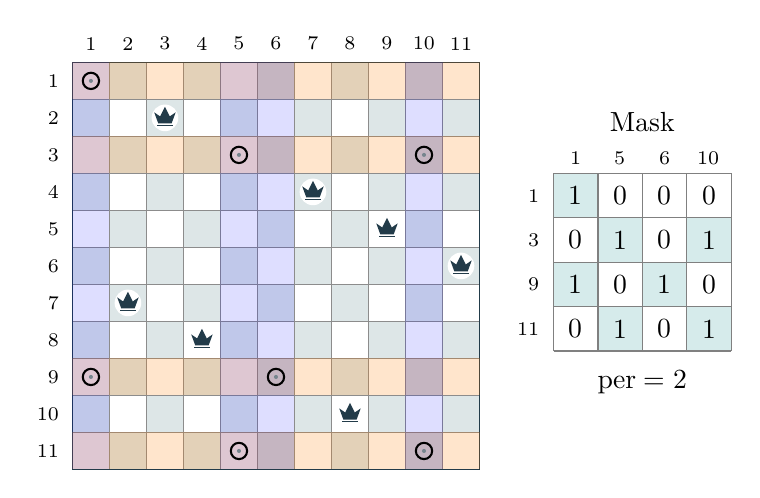
\begin{tikzpicture}[x=.47cm,y=.47cm]
 \bcuadricula{11}
 \foreach \rr in {1,3,9,11}{\fill[orange,opacity=.20] (0,{11-\rr}) rectangle (11,{12-\rr});}
 \foreach \cc in {1,5,6,10}{\fill[blue,opacity=.13] ({\cc-1},0) rectangle (\cc,11);}
 \foreach \rr/\cc in {1/1,3/5,3/10,9/1,9/6,11/5,11/10}{
  \bmarca{11}{\rr}{\cc}
  \draw[black,line width=.75pt] ({\cc-.5},{11.5-\rr}) circle[radius=.22];
 }
 \foreach \rr/\cc in {2/3,4/7,5/9,6/11,7/2,8/4,10/8}{\breina{11}{\rr}{\cc}}
 \begin{scope}[shift={(13,3.2)},scale=1.2]
  \node at (2,5.15) {Mask};
  \foreach \indice/\original in {1/1,2/5,3/6,4/10}
   {\node[font=\scriptsize] at ({\indice-.5},4.35) {$\original$};}
  \foreach \indice/\original in {1/1,2/3,3/9,4/11}
   {\node[font=\scriptsize,anchor=east] at (-.1,{4.5-\indice}) {$\original$};}
  \foreach \rr/\cc in {1/1,2/2,2/4,3/1,3/3,4/2,4/4}
   {\fill[teal!16] ({\cc-1},{4-\rr}) rectangle (\cc,{5-\rr});}
  \draw[step=1,gray,line width=.45pt] (0,0) grid (4,4);
  \foreach \rr/\valores in {1/{1,0,0,0},2/{0,1,0,1},3/{1,0,1,0},4/{0,1,0,1}}{
   \foreach \valor [count=\cc] in \valores
    {\node at ({\cc-.5},{4.5-\rr}) {$\valor$};}
  }
  \node at (2,-.7) {$\operatorname{per}=2$};
 \end{scope}
\end{tikzpicture}
\caption{Board of order eleven for the solution $\pi=(1,3,5,7,9,11,2,4,6,8,10)$ after removing
the queens in rows $1,3,9,11$. Rows are numbered from one, top to bottom, and columns from one, left
to right. Seven queens remain, shown as crowns. The bands highlight the four empty rows and the
empty columns $1,5,6,10$. The circled dots mark the available squares and correspond to the entries
equal to one in the mask, which retains the original labels. Row $1$ forces column $1$, and row $9$
then forces column $6$. Rows $3$ and $11$ can exchange $5$ and $10$, so the permanent is $2$. The positive
differences between rows are $2,6,8,10$, and those between columns are $1,4,5,9$. Since the two
sets are disjoint, no two empty crossings share a diagonal.}\label{fig:terminal}
\end{figure}


Recall that $F$ is the permanence event of Definition~\ref{def:regular}: the history reaches size
$K$, and all its boards, including the arrival board $B^{(K)}$, are regular. The figure illustrates the
geometry. In it, row 1 forces column 1, so every doubly stochastic matrix supported on the mask
assigns
zero mass to the available square $(9,1)$. The example lies outside $F$. Let $D_K$ be the event
that two distinct empty crossings of the board of size $K$ lie on the same diagonal of the initial
board. For $m\ge 1$, write $(u)_m=u(u-1)\cdots(u-m+1)$ if $u\ge m$, and $(u)_m=0$ if $0\le u<m$.

\begin{lema}[Shared diagonals on the last board]\label{terminal-geometria}
Under $\nu$ and under the law $\mu$ of a uniform solution revealed in an independent uniform order,
respectively, we have
\[
 \nu(F\cap D_K)\le d_{n,K}:=\frac{C K^4}{n}\,e^{C'/K},
 \qquad \mu(D_K\mid\pi)\le \frac{C K^4}{n}
\]
for every solution $\pi$. The second probability is taken over the order in which the rows
are revealed.
\end{lema}
\begin{proof}
The initial board has at most $Cn^3$ pairs of distinct squares sharing a diagonal. There are
$n^2$ choices for the first square and at most $2(n-1)$ choices for the second on its diagonals.
For both squares of a pair to be empty crossings at size $K$, two distinct rows and two distinct
columns must remain empty. On $F$ there was no earlier exit, so \eqref{prescr} with $s=t=2$
bounds the probability for each pair by $(K/n)^4e^{C'/K}$. A union bound gives the first claim.

For the second claim, fix $\pi$. The last $K$ rows in the uniform order form a uniform subset $I$
of size $K$. The corresponding columns are $\pi(I)$, and the empty crossings form $I\times\pi(I)$.
Figure~\ref{fig:testigos} shows how the row labels enter two such crossings.
\begin{figure}[htbp]
\centering
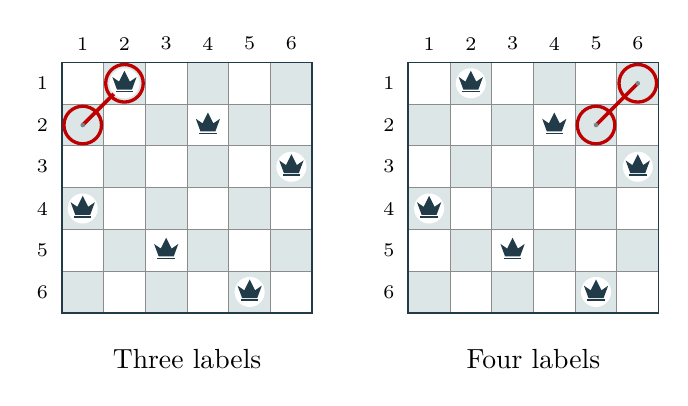
\begin{tikzpicture}[x=.53cm,y=.53cm]
 \foreach \tipo/\dx/\uno/\dos in {3/0/2/1,4/8.3/6/5}{
  \begin{scope}[shift={(\dx,0)}]
   \bcuadricula{6}
   \draw[red!75!black,line width=1.3pt] ({\uno-.5},5.5) -- ({\dos-.5},4.5);
   \bmarca{6}{1}{\uno}
   \bmarca{6}{2}{\dos}
   \draw[red!75!black,line width=1.2pt] ({\uno-.5},5.5) circle[radius=.45];
   \draw[red!75!black,line width=1.2pt] ({\dos-.5},4.5) circle[radius=.45];
   \foreach \rr/\cc in {1/2,2/4,3/6,4/1,5/3,6/5}{\breina{6}{\rr}{\cc}}
   \ifnum\tipo=3
    \node at (3,-1.1) {Three labels};
   \else
    \node at (3,-1.1) {Four labels};
   \fi
  \end{scope}
 }
\end{tikzpicture}
\caption{Two witnesses on the board of order six for the solution $\pi=(2,4,6,1,3,5)$. Rows
are numbered from one, top to bottom, and columns from one, left to right. The crowns are the
queens of $\pi$. Two circles joined by a line mark the squares $(i,\pi(j))$ and $(i',\pi(j'))$
that share a diagonal. On the left, $(i,i',j,j')=(1,2,1,4)$ marks $(1,2)$ and $(2,1)$ and uses
three distinct labels. On the right, $(1,2,3,6)$ marks $(1,6)$ and $(2,5)$ and uses four. With
only two labels we would have $\{i,i'\}=\{j,j'\}$ and $|i-i'|=|\pi(i)-\pi(i')|>0$, in which
case two queens of the solution would attack one another.}\label{fig:testigos}
\end{figure}


A pair sharing a diagonal has the form $(i,\pi(j)),(i',\pi(j'))$, with
\[
 |i-i'|=|\pi(j)-\pi(j')|>0,\qquad i,i',j,j'\in I.
\]
We call a quadruple of labels $(i,i',j,j')$ satisfying this equality of distances a \emph{witness},
whether or not its labels belong to $I$. Put $m=|\{i,i',j,j'\}|$. If $m=2$, the label pairs
$\{i,i'\}$ and $\{j,j'\}$ coincide. The equality of distances would imply that the queens of
$\pi$ in rows $i,i'$ attack each other, which is impossible. If $m=3$, fix $i,i'$ and specify
which of the two labels repeats and in which position $j,j'$ it occurs. The image of that label
under $\pi$ is known. The other image must be at distance $|i-i'|$ from it and hence has at most
two possible values. Each value determines its label via $\pi^{-1}$. Thus there are $O(n^2)$
three-label witnesses. For $m=4$, fixing $i,i',j$ leaves at most two possible values of $\pi(j')$,
giving $O(n^3)$ witnesses.

The subset $I$ contains $m$ fixed labels with probability $(K)_m/(n)_m\le(K/n)^m$ when $n\ge m$.
For $n\ge4$ a union bound gives
\[
 \mu(D_K\mid\pi)\le C\left[n^2(K/n)^3+n^3(K/n)^4\right]\le CK^4/n.
\]
Under $\mu$ the solution and the order can also be completed for histories that have already
stopped. Since $F\cap D_K\subseteq D_K$, integrating the estimate over $\pi$ also gives
$\mu(F\cap D_K)\le CK^4/n$.
\end{proof}

\begin{lema}[Reduction to rooks on the last board]\label{terminal-pivotes}
Let $A$ be the mask of the board $B^{(K)}$. On $F\cap D_K^c$ there is a placement completing the
board, and
\[
 Q(B^{(K)})=\per A,\qquad L(B^{(K)})=L_T(A),
\]
where $L_T(A)=H_T(p)+\log\Gamma_2$ is the rook predictor on the same support, as in the
masked rook model of~\cite[Sections~8.1 and~8.5]{pred}. Here
$H_T(p)=-\sum_e p_e\log p_e+\sum_e(1-p_e)\log(1-p_e)$ is the rook entropy, evaluated at its
stationary point with row and column masses equal to one, and $\Gamma_2$ is the factor from
Section~\ref{costes:permanente}.
\end{lema}
\begin{proof}
On $F$ the Bethe point $p$ of $B^{(K)}$ has row and column masses equal to one and is positive on all
available squares. For any set $I$ of rows, its entire mass $|I|$ goes to the set of neighboring
columns, which admits at most one unit per column. Consequently $|\mathcal N(I)|\ge|I|$.
To see directly that every row can be covered, take a matching of maximum cardinality. If it
leaves a row uncovered, start from all uncovered rows and follow alternating paths, taking
unmatched edges from rows and matched edges from columns. A reachable uncovered column would give
an augmenting path, a contradiction. Every reachable column is therefore matched to a reachable
row, and these matched rows do not exhaust the reachable rows, which include an uncovered row.
Every neighbor of a reachable row is reachable, including the column from which that row was
entered, if any. This contradicts the inequality for the set of reachable rows. Thus $\per A>0$.

On $D_K^c$ each diagonal contains at most one empty crossing. Every permutation on the support
therefore satisfies the constraints from both diagonal families. Moreover, squares on occupied
diagonals were already excluded when forming $A$, so every permutation on the support gives a
legal completion of $B^{(K)}$. The construction is reversible and proves $Q(B^{(K)})=\per A$.

On a free diagonal with one available square $e$, the vacancy is $h_f=1-p_e=:q_e$. Each square
lies on two such diagonals, and a free diagonal with no squares has $h_f=1$. Thus in $H_B$ the
diagonal terms subtract two copies of $\sum_e q_e\log q_e$, leaving exactly the rook entropy
\[
 H_T(p)=-\sum_e p_e\log p_e+\sum_e q_e\log q_e .
\]
The stationarity equation of Lemma~\ref{coste-vacancias} becomes $p_eq_e=a_ib_j$ on every
available square, with the same $a_i,b_j$. The equality $H_B=H_T$ also follows directly as an
identity of functionals at the feasible points on the support, since on every single-square
diagonal the vacancy is always the complement of the sole entry. Hence the Bethe point is also
the stationary point of the rook predictor.

It remains to verify the normalizer, as in \cite[Section~8.1]{pred}. For a square of mass $p$,
put $q=1-p$, $\tau_d=pq/(1-dp)$, and $b_d=(1-dp)/q^d$. When we eliminate the coordinate of its
first diagonal, the pivot in $S_4$ is $q+\tau_4$. If $r$ is the indicator vector of the other lines
of the square,
the Schur complement replaces the contribution $\tau_4rr^T$ in the remaining block by
$(\tau_4-\tau_4^2/(q+\tau_4))rr^T$. We then eliminate the second diagonal of that square with
$d=3$. At both steps,
\[
 q+\tau_d=\frac{q(1-(d-1)p)}{1-dp},\qquad
 \tau_d-\frac{\tau_d^2}{q+\tau_d}=\tau_{d-1},\qquad
 b_d(q+\tau_d)=b_{d-1}.
\]
Since the eliminated diagonal contains a single square, the operation affects only that square's
contribution. A line with no squares has pivot one and does not affect the other coordinates.
The zero mode $(\mathbf1_R,-\mathbf1_C,0)$ has zero coordinate on every eliminated line. We may
therefore calculate the pseudodeterminant in an orthonormal basis of its orthogonal complement
that includes the coordinate vectors of the eliminated diagonals. In this basis the ordinary
factorization using the pivots is exact, and the row and column mode retains its length
$\sqrt{2K}$. The corresponding factor in the normalizer is $\sqrt{2\pi}\sqrt{2K}=\sqrt{4\pi K}$
both before and after elimination. Since $e^{C_d}=\prod_e b_d(p_e)$, the identities prove
$e^{C_4}\pdet S_4=e^{C_2}\pdet S_2$ after the two eliminations per square. In particular,
$\Gamma_4=\Gamma_2$. This gives $L(B^{(K)})=H_T(p)+\log\Gamma_2=L_T(A)$.
\end{proof}

\subsection{Diffusion, scaling, and the determinant}\label{permanente}

In this subsection $K$ is the order of a doubly stochastic matrix $P$, and
$J_K=\mathbf1\mathbf1^T/K$. The estimates also apply with $K=k$ in Section~\ref{costes}.
The outer bounds give constants $M_0$ and $\rho_*<1$ such that
\begin{equation}\label{terminal-hipotesis-matriz}
 0\le P_{ij}\le M_0/K,\qquad \|P-J_K\|_{\rm op}\le\rho_* .
\end{equation}
Indeed, for a doubly stochastic matrix, the row and column block with weights $P$ is
$\left(\begin{smallmatrix}I&P\\P^T&I\end{smallmatrix}\right)$, with eigenvalues $1\pm\sigma_j(P)$.
The two lines of constant vectors correspond to the singular value one. A gap $\gamma>0$ off
the zero mode implies that the remaining singular values are at most $1-\gamma$, which is
precisely the required bound for $P-J_K$.

\begin{lema}[Doubly stochastic scaling]\label{terminal-escalado}
Suppose \eqref{terminal-hipotesis-matriz} holds, and write
$W_{ij}=P_{ij}(1-P_{ij})$ and $a_K=\sum_{ij}P_{ij}^2$. For all sufficiently large $K$, there are
vectors $\alpha,\beta$ with $\sum_i\alpha_i=\sum_j\beta_j$ such that the matrix with entries
$D_{ij}=e^{\alpha_i+\beta_j}W_{ij}$ is doubly stochastic. Moreover,
\[
 \max\{\|\alpha\|_\infty,\|\beta\|_\infty\}=O(K^{-1}),\qquad
 \sum_i\alpha_i+\sum_j\beta_j=a_K+O(K^{-1}),\qquad
 \|D-P\|_{\rm HS}=O(K^{-1}).
\]
The constants depend only on $M_0,\rho_*$. The support of $D$ coincides with that of $P$.
\end{lema}
\begin{proof}
To control the accuracy of the scaling, treated in general in \cite{sk}, consider $S=PP^T$.
It is symmetric and doubly stochastic, with $S_{ij}\le M_0/K$ and $\|S-J_K\|_{\rm op}\le\rho_*^2$,
since $S-J_K=(P-J_K)(P-J_K)^T$. Each row of $S-J_K$ has squared Euclidean norm
$\sum_j S_{ij}^2-1/K\le (M_0-1)/K$. Since $S^t-J_K=(S-J_K)^t$ for every integer $t\ge1$,
multiplying a row of $S-J_K$ by $(S-J_K)^{t-1}$ and passing from the Euclidean norm to the sum
of absolute values gives
\[
 \|S^t-J_K\|_{\infty\to\infty}
 \le \sqrt{M_0-1}\,\rho_*^{\,2(t-1)} .
\]
On mean-zero vectors, the series $\sum_{t\ge0}S^t$ is therefore the inverse of $I-S$, with
uniformly bounded $\infty\to\infty$ norm. The same proof with $P^TP$ gives the bound for
$(I-P^TP)^{-1}$ on this subspace.

Put $S_0=\left(\begin{smallmatrix}I&P\\P^T&I\end{smallmatrix}\right)$.
On the subspace $\sum x=\sum y$, consider the equation $S_0(x,y)=(f,g)$ for $\sum f=\sum g$.
If $s=K^{-1}\sum f$, elimination in the two blocks gives
\[
 \begin{aligned}
 x&=\tfrac12s\mathbf1+(I-PP^T)^{-1}(f-Pg),\\
 y&=\tfrac12s\mathbf1+(I-P^TP)^{-1}(g-P^Tf).
 \end{aligned}
\]
The arguments of both inverses have mean zero. The constant part comes from the fact that $x+Py=f$ and
$y+P^Tx=g$ both have mean $s$ and the means of $x,y$ agree. Since
$\|P\|_{\infty\to\infty}=\|P^T\|_{\infty\to\infty}=1$, the inverse $T$ of $S_0$ in this gauge
satisfies $\|T\|_{\infty\to\infty}\le C_1(M_0,\rho_*)$.

Let $\Psi(\alpha,\beta)$ be the vector of row and column sums of
$(e^{\alpha_i+\beta_j}W_{ij})$ minus one in each coordinate. The sums of its two blocks are
equal. At zero the defect is at most $M_0/K$ by $\sum_jP_{ij}^2\le M_0/K$ and its column
analogue. On a ball of radius $r\le1$, the diagonal blocks of the derivative of $\Psi$
contain the row and column sums of the matrix scaled at the point in question. The off-diagonal
blocks are that matrix and its transpose. In each row and column we have
\[
 \sum_j\big|e^{\alpha_i+\beta_j}W_{ij}-P_{ij}\big|
 \le C_2(r+K^{-1})\sum_jP_{ij}=C_2(r+K^{-1}),
\]
with the same inequality on summing over $i$. Here we used $|\alpha_i+\beta_j|\le2r$ and
$P_{ij}\le M_0/K$. Thus $\|\Psi'-S_0\|_{\infty\to\infty}\le 2C_2(r+K^{-1})$.

With the gauge fixed, the map $u\mapsto u-T\Psi(u)$ moves the origin by at most $C_1M_0/K$.
Take the closed ball of radius $r=2C_1M_0/K$. For large $K$ the derivative of the map has norm
at most $2C_1C_2(r+K^{-1})\le1/2$. The map therefore preserves this ball and is a contraction.
Its fixed point solves $\Psi=0$ and has norm $O(K^{-1})$. Since $P_{ij}<1$ for large $K$, the
factor $(1-P_{ij})e^{\alpha_i+\beta_j}$ is positive and preserves the support.

Uniformly in the indices, we now have
\[
 D_{ij}=P_{ij}\bigl(1+\alpha_i+\beta_j-P_{ij}+O(K^{-2})\bigr).
\]
Sum over $i,j$. Since both $D$ and $P$ have total mass $K$ and the rows and columns of $P$ sum
to one, we obtain $\sum_i\alpha_i+\sum_j\beta_j-a_K=O(K^{-1})$. Also,
$|D_{ij}-P_{ij}|\le C_3P_{ij}/K$ and $a_K\le M_0$. Squaring and summing proves the claim in
Hilbert--Schmidt norm.
\end{proof}

\begin{proposicion}[Permanent of the auxiliary matrix]\label{terminal-permanente}
For the matrices of Lemma~\ref{terminal-escalado}, put $B=P-J_K$. Uniformly under
\eqref{terminal-hipotesis-matriz}, we have
\[
 \log\frac{\per W}{\prod_{ij}(1-P_{ij})}
 =\tfrac12\log(2\pi K)-\tfrac12a_K
   -\tfrac12\log\det(I-B^TB)+o(1).
\]
\end{proposicion}
\begin{proof}
We use McCullagh's estimate~\cite{mccullagh} in the form of \cite[Proposition~3.1]{dw}. If
$D=J_K+B_D$ is doubly stochastic, $\max_{ij}|B_{D,ij}|\le A_0/K$, and $\|B_D\|_{\rm op}\le\rho_0<1$,
then
\[
 \frac{K^K\per D}{K!}=(1+o(1))\det(I-B_D^TB_D)^{-1/2}.
\]
In \cite[Section~2.1]{dw} a doubly stochastic matrix is nonnegative with row and column sums
equal to one, so zero entries are allowed. Divoux and Wang prove the estimate with a relative
error tending to zero uniformly over the class of matrices with fixed bounds $A_0,\rho_0$
\cite[Remark~2.1]{dw}, which is the form we need. Uniformity also follows from the statement
for sequences with one matrix of each order. If uniformity failed, there would be an $\epsilon>0$
and increasing orders $K_j$ with matrices in this class having relative error at least $\epsilon$.
Taking $J_K$ at each remaining order $K$ would give a sequence with the same two bounds for which
the cited proposition would fail.

Let $D$ be the scaling from Lemma~\ref{terminal-escalado}. Since $D_{ij}=P_{ij}(1+O(K^{-1}))$,
its entries are bounded by $C/K$, and $\max|B_{D,ij}|\le A_0/K$. Fix $\rho_*<\rho_0<1$. Then
\[
 \|B_D\|_{\rm op}\le\|P-J_K\|_{\rm op}+\|D-P\|_{\rm HS}
       \le\rho_0
\]
uniformly for all sufficiently large $K$. Moreover, $\|B\|_{\rm HS}^2=a_K-1=O(1)$ and
$\|B_D\|_{\rm HS}=O(1)$. Using $\|X^TY\|_1\le\|X\|_{\rm HS}\|Y\|_{\rm HS}$ for the trace norm gives
\[
 \|B_D^TB_D-B^TB\|_1
 \le(\|B_D\|_{\rm HS}+\|B\|_{\rm HS})\|D-P\|_{\rm HS}
 =O(K^{-1}).
\]
For every point $H$ on the segment between the two Gram matrices, $0\le H\le\rho_0^2I$. The
derivative of $\log\det(I-H)$ in direction $U$ is $-\operatorname{tr}((I-H)^{-1}U)$, whose
absolute value is at most $\|U\|_1/(1-\rho_0^2)$. Integrating along the segment allows us to
replace $B_D$ by $B$ in the logarithm of the determinant, with error $O(K^{-1})$.

Scaling multiplies the product for each permutation by the same factor $\exp(\sum\alpha+\sum\beta)$.
Hence
\[
 \log\per W=\log\per D-a_K+O(K^{-1}).
\]
Finally, $\sum_{ij}P_{ij}=K$, $\sum_{ij}P_{ij}^3=O(K^{-1})$, and Taylor's formula gives
$-\sum_{ij}\log(1-P_{ij})=K+a_K/2+O(K^{-1})$. Applying the cited estimate to $D$ and using
$\log(K!/K^K)=-K+\tfrac12\log(2\pi K)+O(K^{-1})$ gives the asserted formula. All perturbations
and the choice of $A_0,\rho_0$ are uniform for the parameters in \eqref{terminal-hipotesis-matriz}.
\end{proof}

\begin{lema}[Identification with the rook factor]\label{terminal-normalizador}
With the weights of Lemma~\ref{terminal-escalado},
\[
 \log\frac{\per W}{\prod_{ij}(1-P_{ij})}=\log\Gamma_2+o(1)
\]
uniformly under \eqref{terminal-hipotesis-matriz}.
\end{lema}
\begin{proof}
For $S_0=\left(\begin{smallmatrix}I&P\\P^T&I\end{smallmatrix}\right)$, the eigenvalues on the
two lines of constant vectors are two and zero. On their orthogonal complement the singular values
of $P-J_K$ give the factors $(1-\sigma)(1+\sigma)$. Hence
\[
 \pdet S_0=2\det(I-B^TB).
\]
The rook incidence block is $S_2=S_0+\Delta$, where, writing $\iota_e$ for the indicator vector
of the row and column of square $e$, we have
\[
 \Delta=\sum_e\bigl(\tau_2(P_e)-P_e\bigr)\iota_e\iota_e^T,\qquad
 \tau_2(P_e)-P_e=\frac{P_e^2}{1-2P_e}.
\]
The matrix $\Delta$ is positive semidefinite and annihilates the zero mode. The absolute row sums
of $\Delta$ are $O(K^{-1})$ because $P$ is doubly stochastic and $P_{ij}\le M_0/K$, so
$\|\Delta\|_{\rm op}=O(K^{-1})$. Moreover,
$\operatorname{tr}\Delta=2\sum_e P_e^2/(1-2P_e)=2a_K+O(K^{-1})$ and
$\|\Delta\|_{\rm HS}^2\le\|\Delta\|_{\rm op}\operatorname{tr}\Delta=O(K^{-1})$.

On the orthogonal complement of its zero mode, $S_0$ has a gap of at least $1-\rho_*$. On this
subspace put $X=S_0^{-1/2}\Delta S_0^{-1/2}$. We have $X\ge0$ and $\|X\|_{\rm HS}^2=O(K^{-1})$.
Applying $|\log(1+x)-x|\le x^2/2$ for $x\ge0$ gives
\[
 \log\pdet S_2-\log\pdet S_0
 =\operatorname{tr}(S_0^+\Delta)+O(K^{-1}).
\]
To estimate the trace, observe that $\|S_0^+-I\|_{\rm HS}=O(1)$. This is immediate on the
two lines of constant vectors. On their orthogonal complement, $S_0-I$ has off-diagonal blocks
$B,B^T$ and hence Hilbert--Schmidt norm $O(1)$. Multiplication by the bounded inverse $-S_0^{-1}$
gives $S_0^{-1}-I$ on that subspace. The Cauchy--Schwarz inequality for the trace now gives
\[
 |\operatorname{tr}((S_0^+-I)\Delta)|\le
 \|S_0^+-I\|_{\rm HS}\|\Delta\|_{\rm HS}=O(K^{-1/2}).
\]
In conclusion,
\[
 \log\pdet S_2=\log 2+\log\det(I-B^TB)+2a_K+O(K^{-1/2}).
\]
The local term is
$C_2=\sum_{ij}(\log(1-2P_{ij})-2\log(1-P_{ij}))=-a_K+O(K^{-1})$.
Substituting both expansions into
$\log\Gamma_2=(\log(4\pi K)-C_2-\log\pdet S_2)/2$
recovers the right-hand side of Proposition~\ref{terminal-permanente} up to a uniform $o(1)$ error.
\end{proof}

\begin{proposicion}[Error on the last board]\label{terminal-error}
There is a sequence $\theta_K\to0$, depending only on the outer bounds, such that on $F\cap D_K^c$,
\[
 |\log Q(B^{(K)})-L(B^{(K)})|\le\theta_K .
\]
If $G=F\cap\{Q(B^{(K)})>0\}$, then $\nu(G)\ge\nu(F)-d_{n,K}$. For $L_K^{\max}=C K\log(K+1)$
and $\nu(G)>0$, we have
\[
 \begin{aligned}
 \E_\mu\!\left[|g(B^{(K)})|\mathbf1_F\right]
 &\le\theta_K+(L_K^{\max}+\log K!)\, CK^4/n,\\
 \E_{\nu(\cdot\mid G)}[g(B^{(K)})^-]
 &\le\theta_K+L_K^{\max}\,d_{n,K}/\nu(G).
 \end{aligned}
\]
Here $u^-=\max\{-u,0\}$.
\end{proposicion}
\begin{proof}
On $F\cap D_K^c$ take $P=(p_{ij})$ to be the Bethe point, extended by zero off the support of
$A$. Lemma~\ref{terminal-pivotes} gives $H_B=H_T$, $L=H_T+\log\Gamma_2$, and $Q(B^{(K)})=\per A>0$.
The rook stationarity equation gives $W_{ij}=a_i b_j$ on the entire support of $A$. Let
$\mathcal K_T=\prod_i a_i\prod_j b_j$. Multiplying the weights along each permutation and summing
gives $\per W=\mathcal K_T\,\per A$. Use $P_{ij}$ to weight the logarithms of
$P_{ij}(1-P_{ij})=a_i b_j$ on the available squares. Since the row
and column masses equal one, this gives
\[
 H_T(P)=-\log\mathcal K_T+\sum_{ij}\log(1-P_{ij}).
\]
Consequently,
\[
 \log\per A-H_T(P)
 =\log\frac{\per W}{\prod_{ij}(1-P_{ij})}.
\]
Lemma~\ref{terminal-normalizador} gives the first conclusion by uniformity over the possible boards
on $F$. In particular, $F\cap D_K^c\subseteq G$, so $\nu(G)\ge\nu(F)-d_{n,K}$ by
Lemma~\ref{terminal-geometria}.

On the remainder of $F$ we use the entropy of the full predictor directly. In each row,
$-\sum_j p_{ij}\log p_{ij}\le\log K$, while $0\le -(1-y)\log(1-y)\le y$ for $0\le y\le1$.
Summing over squares and diagonals, with $\sum_e p_e=K$ and $\sum_f\ell_f=2K$, gives
\[
 -3K\le H_B(p)\le K\log K+2K .
\]
Lemma~\ref{coste-estatico} then gives $|L(B^{(K)})|\le L_K^{\max}$ for all sufficiently large $K$.
For a history that can be completed, $1\le Q(B^{(K)})\le K!$, so $|g(B^{(K)})|\le L_K^{\max}+\log K!$
and $g(B^{(K)})^-\le L_K^{\max}$.

Under $\mu$ the histories can always be completed. We apply the first conclusion on $F\cap D_K^c$
and the last absolute bound on $F\cap D_K$, whose probability is at most $CK^4/n$ by averaging
Lemma~\ref{terminal-geometria} over $\pi$. Under $\nu(\cdot\mid G)$ the history can also be
completed, and the probability of $D_K$ is at most $\nu(F\cap D_K)/\nu(G)\le d_{n,K}/\nu(G)$.
The first conclusion on $D_K^c$ and the bound on $g^-$ on $D_K$ give the second inequality.
\end{proof}

\section{Final comparison of the counts}\label{balance}
\begin{figure}[htbp]
\centering
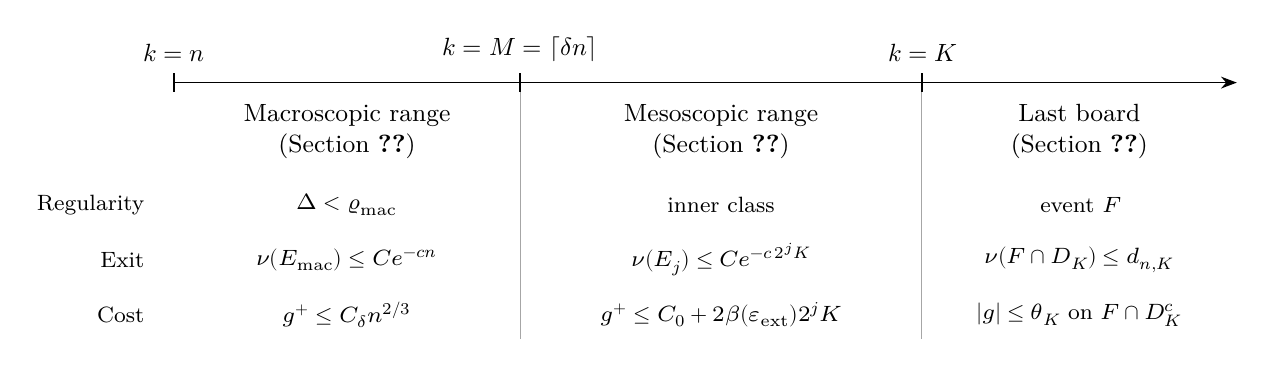
\begin{tikzpicture}[x=1cm,y=1cm,>=Stealth]
 \draw[->,line width=.6pt] (0,0) -- (13.5,0);
 \foreach \x/\lab in {0/{k=n},4.4/{k=M=\lceil\delta n\rceil},9.5/{k=K}}{
  \draw[line width=.6pt] (\x,.12) -- (\x,-.12);
  \node[above,font=\small] at (\x,.14) {$\lab$};
 }
 \foreach \x in {4.4,9.5}{\draw[black!35,line width=.3pt] (\x,-.12) -- (\x,-3.25);}
 \node[font=\small,align=center,text width=4.1cm] at (2.2,-.62)
  {Macroscopic range\\ (Section~\ref{macro})};
 \node[font=\small,align=center,text width=4.8cm] at (6.95,-.62)
  {Mesoscopic range\\ (Section~\ref{meso})};
 \node[font=\small,align=center,text width=3.6cm] at (11.5,-.62)
  {Last board\\ (Section~\ref{terminal})};
 \foreach \y/\lab in {-1.55/Regularity,-2.25/Exit,-2.95/Cost}{
  \node[font=\footnotesize,anchor=east] at (-.25,\y) {\lab};
 }
 \node[font=\footnotesize] at (2.2,-1.55) {$\Delta<\varrho_{\rm mac}$};
 \node[font=\footnotesize] at (6.95,-1.55) {inner class};
 \node[font=\footnotesize] at (11.5,-1.55) {event $F$};
 \node[font=\footnotesize] at (2.2,-2.25) {$\nu(E_{\rm mac})\le Ce^{-cn}$};
 \node[font=\footnotesize] at (6.95,-2.25) {$\nu(E_j)\le Ce^{-c\,2^jK}$};
 \node[font=\footnotesize] at (11.5,-2.25) {$\nu(F\cap D_K)\le d_{n,K}$};
 \node[font=\footnotesize] at (2.2,-2.95) {$g^+\le C_\delta n^{2/3}$};
 \node[font=\footnotesize] at (6.95,-2.95)
  {$g^+\le C_0+2\beta(\varepsilon_{\rm ext})2^jK$};
 \node[font=\footnotesize] at (11.5,-2.95) {$|g|\le\theta_K$ on $F\cap D_K^c$};
\end{tikzpicture}
\caption{The three ranges of a history, from left to right as the size $k$ decreases. The first
row gives the regularity condition of Definition~\ref{def:regular}. The second gives the bound on
the exit probability under $\nu$, with the events $E_{\rm mac}$ and $E_j$ of this section
(Corollary~\ref{macro:cambio}, Lemma~\ref{meso:entrada}, and
Proposition~\ref{prop:salida-banda-meso}) and, on the last board, the bound of
Lemma~\ref{terminal-geometria}. The third gives the bound on the cost at the first-exit board
(Proposition~\ref{coste-macro} and Corollary~\ref{coste-debil}) and the bound of
Proposition~\ref{terminal-error}. The constants $C$ and $c$ in the macroscopic range depend on
$\delta$ and $\varrho_{\rm mac}$. Corollary~\ref{hist:consistencia} bounds $A_\tau$ along the whole
history.}\label{fig:tramos}
\end{figure}

\begin{proof}[Proof of Theorem~\ref{princ}]
Fix the class constants, $a_{\rm mes}$, $\varrho_{\rm mes}$ and the tolerances, $\varepsilon$,
$\delta$, $K_0$, $\varrho_{\rm mac}$ and $a_{\rm mac}$ in the order given in
Section~\ref{meso:constantes}. Let $K\ge K_0$ be a fixed integer and let $\tau$ be the stopping
time in Definition~\ref{def:regular}. This stopping time satisfies the hypotheses of
Section~\ref{historias}. Indeed, every parent before $\tau$ is regular and therefore has a Bethe
point with fixed bounds: by Proposition~\ref{macro:maximo} and Corollary~\ref{macro:cambio} in the
macroscopic range, by Proposition~\ref{meso:reconstruccion} at the cut-off, and by definition in
the mesoscopic range. By item (I1) of Section~\ref{leyes}, each of its children has a Bethe point
and a finite predictor. These same bounds are the hypotheses of
Corollary~\ref{hist:consistencia}. Let $E_{\rm mac}$ be the event that the first-exit board has
size ${k\ge M}$; this includes failure of entry at the cut-off $k=M$. For $j\ge0$, let $E_j$ be
the event that the history has regular entry at $M$ and its first-exit board has size $k$ with
${2^jK\le k<2^{j+1}K}$; this is the event in Proposition~\ref{prop:salida-banda-meso}. If $K<M$,
an exit on the board of size $K$ belongs to $E_0$. These events and the permanence event $F$
partition the stopped histories.

On $E_{\rm mac}$ and on each $E_j$, the first-exit board $B_\tau$ inherits the outer bounds from
its regular parent; on $E_j$ it also inherits diagonal mass at most $\varepsilon_{\rm ext}$
(Proposition~\ref{meso:reconstruccion}). On $E_{\rm mac}$ its size is $k\ge M\ge\delta n$, so
$N=2n-1=O_\delta(k)$ and Proposition~\ref{coste-macro} bounds its exit cost by
$\Lambda_{\rm mac}=C_\delta n^{2/3}$. On $E_j$, writing $k$ for its size,
Corollary~\ref{coste-debil} gives
\[
 g(B_\tau)\le C_0+\beta(\varepsilon_{\rm ext})k
           \le C_0+2\beta(\varepsilon_{\rm ext})2^jK=:\Lambda_j .
\]
Both bounds hold on histories of positive mass under $\mu$. Let $\Lambda$ be the function of the
stopped history equal to $\Lambda_{\rm mac}$ on $E_{\rm mac}$, to $\Lambda_j$ on $E_j$, and to zero
on $F$. Thus $g(B_\tau)\mathbf1_{F^c}\le\Lambda$ on these histories.

We apply the Gibbs variational inequality~\cite[Proposition~1.4.2]{de} (see
also~\cite[Ch.~2]{ct}) to $\Lambda$ and to the laws of the stopped
histories. On this finite space the inequality follows directly from Jensen's inequality by
restricting the sum under $\nu$ to the support of $\mu$:
\[
 \E_\mu\Lambda-D(\mu^\tau\Vert\nu^\tau)\le\log\E_\nu e^\Lambda
 =\log\!\left(1+\nu(E_{\rm mac})(e^{\Lambda_{\rm mac}}-1)
              +\sum_{j\ge0}\nu(E_j)(e^{\Lambda_j}-1)\right).
\]
If the first exit occurs at $M$ with $\Delta<\varrho_{\rm mac}$, Lemma~\ref{meso:entrada} places
the observables within their entry tolerances, so $D_{\max}(M)\ge\alpha_{\rm geo} M$. Thus
\[
 E_{\rm mac}\subseteq\mathcal H_M\cup\bigl(G_M^-\cap\{D_{\max}(M)\ge\alpha_{\rm geo} M\}\bigr),
\]
so Corollary~\ref{macro:cambio} and that lemma bound the macroscopic summand by
${C_1\exp(-c_1n+C_\delta n^{2/3})}$, with $C_1,c_1>0$ depending on $\delta$ and $\varrho_{\rm mac}$.
Proposition~\ref{prop:salida-banda-meso} gives ${\nu(E_j)\le C\exp(-c\,2^jK)}$ if $2^jK\le M$;
otherwise $E_j$ is empty. Since $c>2\beta(\varepsilon_{\rm ext})$, for
$0<c'<c-2\beta(\varepsilon_{\rm ext})$ the sum of $\nu(E_j)(e^{\Lambda_j}-1)$ is $O(e^{-c'K})$ for
large $K$. Corollary~\ref{hist:consistencia}, \eqref{super}, and the terminal estimate
under $\mu$ in Proposition~\ref{terminal-error} give
\[
 \limsup_{n\to\infty}g(B_0)\le C/K+\theta_K+Ce^{-c'K},\qquad\theta_K\to0 .
\]
Indeed, for fixed $K$ the exceptional cost on the last board is at most
${(L_K^{\max}+\log K!)\,CK^4/n}$, which is ${O(K^5\log(K+1)/n)}$ and tends to zero before we take
the limit in $K$.

For the reverse inequality we use $G=F\cap\{Q(B^{(K)})>0\}$. By the geometric estimate under $\nu$
in Section~\ref{terminal}, $s=\nu(G)\ge1-Ce^{-cK}-o_n(1)-d_{n,K}$, where $d_{n,K}\to0$ for fixed
$K$. For large $K$ this lower limit is positive. The negative part of the exceptional cost on the
last board has expectation at most $L_K^{\max}d_{n,K}/s$ under $\nu(\cdot\mid G)$. On the remaining
histories $\theta_K$ suffices. Taking the lower limit in \eqref{infer} and using
$\log(1-z)\ge-2z$ for $0\le z\le1/2$ gives
\[
 \liminf_{n\to\infty}g(B_0)\ge-C/K-\theta_K-Ce^{-cK}.
\]
Now let $K$ tend to infinity in both inequalities. On the initial board $B_0$, the global maximizer
in Proposition~\ref{macro:maximo} satisfies $p_{\max}<1/4$ for large $n$ and hence coincides with
the canonical maximizer of~\cite{pred}. The relation between the cofactor and the pseudodeterminant
in Section~\ref{leyes} gives $L(B_0)=\log Q_{\rm pred}(n)$. Thus
$g(B_0)=\log Q(n)-\log Q_{\rm pred}(n)\to0$. Applying Theorem~1.1 of~\cite{pred} to the second
logarithm, which is item (I5), identifies the constant in the statement.
\end{proof}

\section{Discussion}
The reduction to a permanent takes place after the last rows are chosen. The uniform order gives
the geometric bound even for a fixed solution. Under the adaptive law, the same phenomenon follows
from the survival probabilities of prescribed rows and columns. This distinction explains why the
two bounds on the count can use the same last board even though their histories have different
distributions.

The permanent estimate is uniform over a class with fixed diffusion and gap bounds. Its remainder
tends to zero as the size of the last board grows. The order of limits in Section~\ref{balance}
allows us to use precisely this information. The $O(1/n)$ rate in Conjecture~10.1 of~\cite{pred}
remains open. In addition to the permanent error $\theta_K$, the final comparison involves the bound
$C/K+O_\delta(1/n)$ from cumulative consistency (Corollary~\ref{hist:consistencia}), the cost of exits
by band, of order $e^{-c'K}$, and the exceptional contribution of the last board, of order
$K^5\log(K+1)/n$ (Proposition~\ref{terminal-error}). With these bounds, no choice of $K$ as a
function of $n$ gives the rate: $C/K=O(1/n)$ requires $K\ge cn$, in which case
$K^5\log(K+1)/n$ does not tend to zero. To obtain the rate by this method one would have to improve
these bounds and control the permanent error when choosing the floor $K$, or justify cancellations
among the contributions.

There are two close precedents for a result of this type. Eberhard, Manners and
Mrazović~\cite{emm} obtained the asymptotic equivalent of the number of placements of semiqueens
on the toroidal board by a version of the circle method. Tripathi~\cite{tripathi} identifies the
limiting constant of the partition function of a class of Mallows models with a Fredholm
determinant, and also uses McCullagh's estimate~\cite{mccullagh}.

\section*{Use of artificial intelligence tools}
\addcontentsline{toc}{section}{Use of artificial intelligence tools}

Artificial intelligence tools were used to organize the sources, compare versions, prepare the typesetting
and editorial restructuring of the text, and conduct adversarial reviews of text excerpts.

\begin{thebibliography}{99}
\raggedright

\bibitem{bk} C.~Bowtell and P.~Keevash, \emph{The $n$-queens problem}, arXiv:2109.08083v1 (2021).
\href{https://doi.org/10.48550/arXiv.2109.08083}{doi:10.48550/arXiv.2109.08083}.

\bibitem{ct} T.~M.~Cover and J.~A.~Thomas, \emph{Elements of Information Theory}, 2nd ed., Wiley,
2006. \href{https://doi.org/10.1002/047174882X}{doi:10.1002/047174882X}.

\bibitem{dw} A.~Divoux and S.~Wang, \emph{The maximum number of Hamiltonian cycles in tournaments},
arXiv:2610.23755v1 (2026).
\href{https://doi.org/10.48550/arXiv.2610.23755}{doi:10.48550/arXiv.2610.23755}.

\bibitem{ls} Z.~Luria and M.~Simkin, \emph{A lower bound for the $n$-queens problem}, in
\emph{Proceedings of the 2022 Annual ACM-SIAM Symposium on Discrete Algorithms (SODA)}, SIAM, 2022,
2185--2197.
\href{https://doi.org/10.1137/1.9781611977073.86}{doi:10.1137/1.9781611977073.86};
arXiv:2105.11431.

\bibitem{mccullagh} P.~McCullagh, \emph{An asymptotic approximation for the permanent of a doubly
stochastic matrix}, J. Stat. Comput. Simul. \textbf{84} (2014), 404--414.
\href{https://doi.org/10.1080/00949655.2012.712122}{doi:10.1080/00949655.2012.712122};
arXiv:1205.5723.

\bibitem{ultimas} D.~S.~Mejia, \emph{Completability of the Final Layers in the
$n$-Queens Problem}, preprint, Zenodo, 2026, version~1.
\href{https://doi.org/10.5281/zenodo.24221374}{doi:10.5281/zenodo.24221374}.

\bibitem{perfil} D.~S.~Mejia, \emph{The Variational Profile of Partial Queen Placements:
Existence, Euler Equations, and Regularity up to the Full Board}, preprint, Zenodo, 2026,
version~1.
\href{https://doi.org/10.5281/zenodo.24220042}{doi:10.5281/zenodo.24220042}.

\bibitem{pred} D.~S.~Mejia, \emph{The Canonical Predictor for the $n$-Queens Problem:
Constant Term and Consistency}, preprint, Zenodo, 2026, version~1.
\href{https://doi.org/10.5281/zenodo.24241043}{doi:10.5281/zenodo.24241043}.

\bibitem{nab} P.~Nobel, A.~Agrawal and S.~Boyd, \emph{Computing tighter bounds on the $n$-queens
constant via Newton's method}, Optim. Lett. \textbf{17} (2023), 1229--1240.
\href{https://doi.org/10.1007/s11590-022-01933-2}{doi:10.1007/s11590-022-01933-2}.

\bibitem{simkin} M.~Simkin, \emph{The number of $n$-queens configurations}, Adv. Math.
\textbf{427} (2023), 109127.
\href{https://doi.org/10.1016/j.aim.2023.109127}{doi:10.1016/j.aim.2023.109127}. We cite the numbering
of version arXiv:2107.13460v3.

\bibitem{sk} R.~Sinkhorn and P.~Knopp, \emph{Concerning nonnegative matrices and doubly stochastic
matrices}, Pacific J. Math. \textbf{21} (1967), 343--348.
\href{https://doi.org/10.2140/pjm.1967.21.343}{doi:10.2140/pjm.1967.21.343}.
\end{thebibliography}

\end{document}
